\documentclass[conference,a4paper]{IEEEtran}
\usepackage[T1]{fontenc}
\usepackage[utf8]{inputenc}
\usepackage{amsmath,amssymb}
\usepackage{graphicx}
\usepackage{booktabs}
\usepackage{array}
\usepackage{url}
\usepackage{fancyvrb}
\usepackage{tikz}
\usetikzlibrary{arrows.meta,positioning,shapes.geometric,patterns}
\usepackage{pgfplots}
\pgfplotsset{compat=1.18}
\usepackage[hidelinks]{hyperref}
\usepackage{cite}
\newcommand{\code}[1]{\texttt{#1}}
\renewcommand{\topfraction}{0.95}\renewcommand{\bottomfraction}{0.8}
\renewcommand{\textfraction}{0.05}\renewcommand{\floatpagefraction}{0.85}
\renewcommand{\dbltopfraction}{0.95}\renewcommand{\dblfloatpagefraction}{0.85}
\setcounter{topnumber}{4}\setcounter{bottomnumber}{2}\setcounter{totalnumber}{6}

\begin{document}

\title{CSE513 Assignment 2: Virtual Memory --- Predict, Simulate, and Observe}
\author{Şevval İLHAN\\[2pt]
\normalsize Student No. 264201001416\\
Source code: submitted as \code{cse513-a2.zip}\\
14 November 2026}
\maketitle

\begin{abstract}
This report studies how address translation, page replacement and memory access patterns affect execution. Six virtual-address accesses are traced by hand through a page table, distinguishing normal accesses, demand paging, copy-on-write and protection or mapping failures. The supplied page-replacement simulator is extended with read/write operations, dirty bits, writeback and transfer-cost accounting, strict input validation and run-time verification of invariants. The first eight steps of Workload~A under FIFO, LRU, OPT and CLOCK and all twelve steps of Workload~B under FIFO with three and four frames were calculated by hand and agree with the simulator in every decision. Two additional tests show when a dirty bit is retained and reset, and that two policies with equal fault counts can differ by 33\,\% in modeled time. Thirty automated checks, a differential comparison with an independent reference model on 2{,}000 random workloads and five injected bugs support the correctness of the implementation. Finally, demand paging and copy-on-write are observed on Ubuntu~24.04, where every observation matched its prediction.
\end{abstract}

\begin{IEEEkeywords}
Virtual memory, address translation, page replacement, dirty page, copy-on-write, demand paging, Belady's anomaly.
\end{IEEEkeywords}

\section{Introduction}
A process addresses memory through virtual addresses, which the hardware translates through a page table into physical frames \cite{silberschatz}. When a translation cannot be completed, the operating system decides whether the access can be repaired---by loading the page (demand paging) or by giving the process its own copy (copy-on-write, COW)---or whether it must be refused. When memory is full, a replacement policy chooses which resident page to evict, and a modified (dirty) victim must first be written back.

The assignment \cite{handout} combines these questions at three levels: hand tracing of individual addresses, simulation of replacement policies with a cost model, and observation of real behaviour on Ubuntu. Section~\ref{sec:addr} presents the six address cases, Section~\ref{sec:design} the simulator extension, Section~\ref{sec:traces} the hand traces and their comparison with the simulator, Section~\ref{sec:cost} the cost results, and Section~\ref{sec:tests} the student-designed tests. Section~\ref{sec:verif} describes the verification, Section~\ref{sec:analysis} answers the analysis questions, and Section~\ref{sec:ubuntu} reports the Ubuntu experiments. The scanned hand calculations are reproduced in the Appendix.

\section{Address Translation}\label{sec:addr}
\subsection{Method}
Pages are 4\,KiB (4096 bytes) and addresses are byte addresses. For a virtual address $VA$,
\begin{align}
\mathit{VPN} &= \lfloor VA / 4096 \rfloor, \label{eq:vpn}\\
\mathit{offset} &= VA \bmod 4096, \label{eq:off}\\
PA &= \mathit{frame} \times 4096 + \mathit{offset}. \label{eq:pa}
\end{align}
Since $4096 = \mathrm{0x1000}$, the low three hexadecimal digits of an address form the offset and the remaining digits the page or frame number, which provides a check on (\ref{eq:vpn})--(\ref{eq:pa}). Each access is treated independently from the initial state, translation is checked through the page table only (no TLB), and the checks are applied in the order of Fig.~\ref{fig:flow}: mapping, permission, presence, and finally whether a permitted write hits a COW-protected page.

\begin{figure}[!tb]
\centering
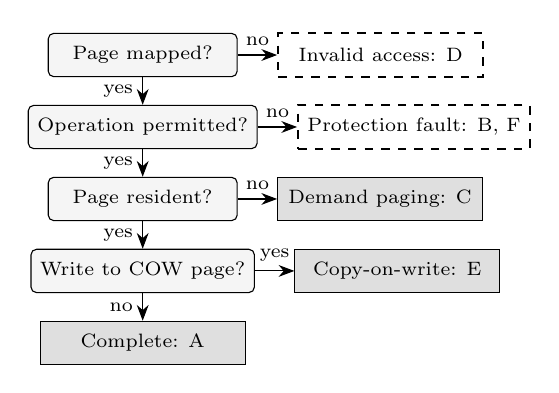
\begin{tikzpicture}[font=\scriptsize, node distance=3.5mm and 3mm,
  q/.style={draw, rounded corners=2pt, align=center, minimum width=2.4cm, minimum height=5.5mm, fill=gray!8},
  ok/.style={draw, align=center, minimum width=2.6cm, minimum height=5.5mm, fill=gray!25},
  bad/.style={draw, align=center, minimum width=2.6cm, minimum height=5.5mm, dashed, thick, fill=white},
  >={Stealth[length=2mm]}]
\node[q] (m) {Page mapped?};
\node[q, below=of m] (p) {Operation permitted?};
\node[q, below=of p] (r) {Page resident?};
\node[q, below=of r] (c) {Write to COW page?};
\node[ok, below=of c] (a) {Complete: A};
\node[bad, right=5mm of m] (d) {Invalid access: D};
\node[bad, right=5mm of p] (bf) {Protection fault: B, F};
\node[ok, right=5mm of r] (cc) {Demand paging: C};
\node[ok, right=5mm of c] (e) {Copy-on-write: E};
\draw[->] (m) -- node[left]{yes} (p);
\draw[->] (p) -- node[left]{yes} (r);
\draw[->] (r) -- node[left]{yes} (c);
\draw[->] (c) -- node[left]{no} (a);
\draw[->] (m) -- node[above]{no} (d);
\draw[->] (p) -- node[above]{no} (bf);
\draw[->] (r) -- node[above]{no} (cc);
\draw[->] (c) -- node[above]{yes} (e);
\end{tikzpicture}
\caption{Order of the checks applied to each access and the outcome of cases A--F. Grey boxes complete (C and E after recovery); dashed boxes fail.}
\label{fig:flow}
\end{figure}

\begin{table*}[!t]
\renewcommand{\arraystretch}{1.15}
\setlength{\tabcolsep}{4.5pt}
\caption{Results of the Six Address Cases}
\label{tab:addr}
\centering\footnotesize
\begin{tabular}{l l r c c l l l}
\toprule
Access & Operation, VA & VA (dec.) & Page & Offset & Event & Outcome & Physical address \\
\midrule
A & Read 0x002A & 42 & 0 & 0x02A (42) & Normal access, no fault & Completes & 0x302A $= 3 \cdot 4096 + 42 = 12330$ \\
B & Write 0x1064 & 4196 & 1 & 0x064 (100) & Protection fault (read-only page) & Fails & none \\
C & Read 0x2040 & 8256 & 2 & 0x040 (64) & Page fault, demand paging & After recovery & 0x6040 $= 6 \cdot 4096 + 64 = 24640$ \\
D & Read 0x3000 & 12288 & 3 & 0x000 (0) & Invalid access (unmapped) & Fails & none \\
E & Write 0x4001 & 16385 & 4 & 0x001 (1) & Copy-on-write fault & After recovery & 0x9001 $= 9 \cdot 4096 + 1 = 36865$ \\
F & Write 0x5008 & 20488 & 5 & 0x008 (8) & Protection fault (read-only page) & Fails & none \\
\bottomrule
\end{tabular}
\end{table*}

\subsection{The Six Accesses}
Table~\ref{tab:addr} summarises the results; the reasoning for each case follows.

\emph{A, read 0x002A.} $\mathrm{0x002A} = 2\times16+10 = 42$, so $\mathit{VPN}=\lfloor 42/4096\rfloor = 0$ and the offset is 42. Page~0 is mapped read and write and resident in frame~3; the read is permitted and completes without a fault at $PA = \mathrm{0x302A}$. No mapping changes, and neither input nor copying is needed.

\emph{B, write 0x1064.} $\mathrm{0x1064} = 4196$, page~1, offset 0x064. Page~1 is resident in frame~5 but read only. The write fails the permission check and raises a protection fault; demand paging and COW do not apply, the write is denied and no physical address is produced. Translating the frame number alone would give 0x5064, but that address is never accessed.

\emph{C, read 0x2040.} $\mathrm{0x2040} = 8256$, page~2, offset 0x040. Page~2 permits reading but is absent, so a page fault occurs. The operating system reads the page from its file into the free frame~6, marks page~2 present in frame~6, and restarts the read, which completes at $PA = \mathrm{0x6040}$. One page input is required; no copy.

\emph{D, read 0x3000.} $\mathrm{0x3000} = 12288$, page~3, offset~0. Page~3 is unmapped and has no backing, so the access is invalid (a segmentation fault on Linux). No physical address exists and nothing changes.

\emph{E, write 0x4001.} $\mathrm{0x4001} = 16385$, page~4, offset~1. Page~4 is a private read-and-write mapping, so the write is permitted, but the page is resident in the shared frame~8 with hardware write access disabled for COW. The write faults; the operating system copies frame~8 into the free frame~9, maps page~4 to frame~9 with write access enabled, retains frame~8 for the other process, and restarts the write at $PA = \mathrm{0x9001}$. One page copy is needed and no disk input.

\emph{F, write 0x5008.} $\mathrm{0x5008} = 20488$, page~5, offset~8. Page~5 is read only, so the write is denied with a protection fault. The page is also absent, but it is not loaded: the permission check fails first, and loading the page would not make the write legal. Page~5 remains absent, and there is no physical address, input or copy.

\subsection{Why Free RAM Cannot Repair an Illegal Access}
Free frames help only when an access is legal but the data is not yet where it must be: in C the page is absent, and in E a shared page must be copied before the private write. Accesses B, D and F fail because the access itself is not allowed---page~3 has no mapping, and pages~1 and~5 do not permit writing. Free memory changes neither the mapping nor the permissions, so however much RAM is available the operating system must refuse these accesses.

Two points in the hand solutions (Appendix, sheets 1--3) were sharpened in this report: in B the sheet computes 0x5064 before stating that no physical address is produced, and in E the sheet does not state explicitly that frame~8 is retained for the other process.

\section{Simulator Design}\label{sec:design}
\subsection{Replacement Model}
The simulator follows the simplified model of the assignment \cite{handout}. There is one process with initially empty, equal-sized frames, and there is no prefetching, sharing, pinning or background writeback. Each reference has a page number (0--999) and an operation, R or W. Every absent reference is a fault that needs one page input, including write misses and the initial fills of empty frames; an initial fill is not an eviction. A loaded page starts clean, a W sets its dirty bit, and an R leaves the bit unchanged, also on a hit. Evicting a dirty page requires one writeback, which is counted only at eviction; dirty pages still resident at the end are reported separately and are not flushed.

FIFO evicts the page inserted longest ago and ignores hits. LRU evicts the least recently accessed page, where both reads and writes update recency. OPT evicts the page whose next reference is farthest in the future; pages never referenced again are farthest, and ties are broken by the lowest frame index. These three policies fill the lowest-index empty frame before evicting. CLOCK starts with the hand at frame~0 and all reference bits 0; on a miss it clears reference bits equal to 1 and advances until it finds an empty frame or a frame with reference bit~0, installs the page there with reference bit~1, and advances the hand once. A hit sets the reference bit without moving the hand. Dirty bits never influence victim selection.

\subsection{Implementation}
The simulator is a C11 command-line program, \code{src/replacement.c}, built on the course-supplied \code{replacement.c}. The supplied victim-selection code---frame search, FIFO insertion times, LRU last-use times, OPT look-ahead with lowest-index tie-break and the CLOCK sweep---is reused unchanged and marked \code{[SUPPLIED]}. The additions, marked \code{[A2]}, are: parsing of \code{page:op} tokens from arguments or a file; strict validation with an explanatory message (exit status~2) for frame counts outside 1--64, sequences that are empty or longer than 256 references, pages outside 0--999 or containing anything other than decimal digits, and operations other than R or W; a dirty bit per frame; counters for hits, faults, initial fills, evictions and dirty writebacks; the cost model of Section~\ref{sec:cost}; and invariant checks after every step and at the end (Section~\ref{sec:verif}).

For every reference the output shows the step, page and operation, hit or fault, the victim or none, whether a dirty writeback occurred, and the page and dirty bit of every frame after the access; for CLOCK it also shows the reference bits and the next hand position. The output is a readable table or, with \code{--csv}, a CSV trace. A summary reports the totals, the resident dirty pages and the modeled time. Build and run instructions, the input format and the known limitations are given in the README.

\section{Workloads and Hand Traces}\label{sec:traces}
Workload~A uses the page sequence of the lecture with added operations,
\begin{center}\footnotesize
\code{7:R 0:W 1:R 2:W 0:R 3:R 0:W 4:R 2:R 3:W}\\
\code{0:R 3:R 2:W 1:R 2:R 0:R 1:W 7:R 0:R 1:R}
\end{center}
and is run with three frames under all four policies. Workload~B,
\begin{center}\footnotesize
\code{1:R 2:R 3:R 4:R 1:R 2:R 5:R 1:R 2:R 3:R 4:R 5:R},
\end{center}
contains only reads and is run with FIFO using three and four frames. Before the program was run, the first eight steps of A under each policy and all steps of B were calculated by hand, including dirty state (Appendix, sheets 4--5).

Tables~\ref{tab:afifo}--\ref{tab:bfifo4} give the complete simulator traces. A check mark in the last column means that the hand-calculated row is identical in every field: hit or fault, victim, writeback, frame contents, dirty bits and, for CLOCK, reference bits and hand. An asterisk marks a dirty page. The rows were compared automatically (Section~\ref{sec:verif}).

\begin{table}[!tb]
\renewcommand{\arraystretch}{1.05}
\setlength{\tabcolsep}{3.2pt}
\caption{FIFO on Workload A, 3 frames: simulator trace (steps 1--8 also calculated by hand)}
\label{tab:afifo}
\centering\footnotesize
\begin{tabular}{r c c r c c c c c}
\toprule
Step & Ref & H/F & Vic. & WB & F0 & F1 & F2 & Hand calc. \\
\midrule
1 & 7:R & F & -- & -- & 7 & -- & -- & \checkmark \\
2 & 0:W & F & -- & -- & 7 & 0$^{\ast}$ & -- & \checkmark \\
3 & 1:R & F & -- & -- & 7 & 0$^{\ast}$ & 1 & \checkmark \\
4 & 2:W & F & 7 & -- & 2$^{\ast}$ & 0$^{\ast}$ & 1 & \checkmark \\
5 & 0:R & H & -- & -- & 2$^{\ast}$ & 0$^{\ast}$ & 1 & \checkmark \\
6 & 3:R & F & 0 & yes & 2$^{\ast}$ & 3 & 1 & \checkmark \\
7 & 0:W & F & 1 & -- & 2$^{\ast}$ & 3 & 0$^{\ast}$ & \checkmark \\
8 & 4:R & F & 2 & yes & 4 & 3 & 0$^{\ast}$ & \checkmark \\
\midrule
9 & 2:R & F & 3 & -- & 4 & 2 & 0$^{\ast}$ &  \\
10 & 3:W & F & 0 & yes & 4 & 2 & 3$^{\ast}$ &  \\
11 & 0:R & F & 4 & -- & 0 & 2 & 3$^{\ast}$ &  \\
12 & 3:R & H & -- & -- & 0 & 2 & 3$^{\ast}$ &  \\
13 & 2:W & H & -- & -- & 0 & 2$^{\ast}$ & 3$^{\ast}$ &  \\
14 & 1:R & F & 2 & yes & 0 & 1 & 3$^{\ast}$ &  \\
15 & 2:R & F & 3 & yes & 0 & 1 & 2 &  \\
16 & 0:R & H & -- & -- & 0 & 1 & 2 &  \\
17 & 1:W & H & -- & -- & 0 & 1$^{\ast}$ & 2 &  \\
18 & 7:R & F & 0 & -- & 7 & 1$^{\ast}$ & 2 &  \\
19 & 0:R & F & 1 & yes & 7 & 0 & 2 &  \\
20 & 1:R & F & 2 & -- & 7 & 0 & 1 &  \\
\bottomrule
\end{tabular}
\end{table}
\begin{table}[!tb]
\renewcommand{\arraystretch}{1.05}
\setlength{\tabcolsep}{3.2pt}
\caption{LRU on Workload A, 3 frames: simulator trace (steps 1--8 also calculated by hand)}
\label{tab:alru}
\centering\footnotesize
\begin{tabular}{r c c r c c c c c}
\toprule
Step & Ref & H/F & Vic. & WB & F0 & F1 & F2 & Hand calc. \\
\midrule
1 & 7:R & F & -- & -- & 7 & -- & -- & \checkmark \\
2 & 0:W & F & -- & -- & 7 & 0$^{\ast}$ & -- & \checkmark \\
3 & 1:R & F & -- & -- & 7 & 0$^{\ast}$ & 1 & \checkmark \\
4 & 2:W & F & 7 & -- & 2$^{\ast}$ & 0$^{\ast}$ & 1 & \checkmark \\
5 & 0:R & H & -- & -- & 2$^{\ast}$ & 0$^{\ast}$ & 1 & \checkmark \\
6 & 3:R & F & 1 & -- & 2$^{\ast}$ & 0$^{\ast}$ & 3 & \checkmark \\
7 & 0:W & H & -- & -- & 2$^{\ast}$ & 0$^{\ast}$ & 3 & \checkmark \\
8 & 4:R & F & 2 & yes & 4 & 0$^{\ast}$ & 3 & \checkmark \\
\midrule
9 & 2:R & F & 3 & -- & 4 & 0$^{\ast}$ & 2 &  \\
10 & 3:W & F & 0 & yes & 4 & 3$^{\ast}$ & 2 &  \\
11 & 0:R & F & 4 & -- & 0 & 3$^{\ast}$ & 2 &  \\
12 & 3:R & H & -- & -- & 0 & 3$^{\ast}$ & 2 &  \\
13 & 2:W & H & -- & -- & 0 & 3$^{\ast}$ & 2$^{\ast}$ &  \\
14 & 1:R & F & 0 & -- & 1 & 3$^{\ast}$ & 2$^{\ast}$ &  \\
15 & 2:R & H & -- & -- & 1 & 3$^{\ast}$ & 2$^{\ast}$ &  \\
16 & 0:R & F & 3 & yes & 1 & 0 & 2$^{\ast}$ &  \\
17 & 1:W & H & -- & -- & 1$^{\ast}$ & 0 & 2$^{\ast}$ &  \\
18 & 7:R & F & 2 & yes & 1$^{\ast}$ & 0 & 7 &  \\
19 & 0:R & H & -- & -- & 1$^{\ast}$ & 0 & 7 &  \\
20 & 1:R & H & -- & -- & 1$^{\ast}$ & 0 & 7 &  \\
\bottomrule
\end{tabular}
\end{table}

\subsection{FIFO on Workload A}
The first three references fill frames 0--2; page~0 becomes dirty at step~2. At step~4, page~7 is the oldest and clean, so it is evicted without a writeback, and the write makes page~2 dirty. Step~5 is a hit that does not change insertion order. At step~6 the oldest page is the dirty page~0, so the first writeback occurs. Page~0 is then needed again at step~7 and must be reloaded clean before the write makes it dirty again, an example of FIFO evicting a heavily used page. At step~8 the dirty page~2 is evicted with the second writeback. Over all 20 references FIFO incurs 15 faults and 6 writebacks (Table~\ref{tab:afifo}).

\subsection{LRU on Workload A}
LRU agrees with FIFO up to step~5, but the hit at step~5 makes page~0 recently used. At step~6 the least recently used page is~1, which is clean, so no writeback is needed, and the write to page~0 at step~7 becomes a hit. At step~8 page~2 (last used at step~4) is evicted with a writeback. Over the whole workload LRU incurs 12 faults and 4 writebacks (Table~\ref{tab:alru}).

\begin{table}[!tb]
\renewcommand{\arraystretch}{1.05}
\setlength{\tabcolsep}{3.2pt}
\caption{OPT on Workload A, 3 frames: simulator trace (steps 1--8 also calculated by hand)}
\label{tab:aopt}
\centering\footnotesize
\begin{tabular}{r c c r c c c c c}
\toprule
Step & Ref & H/F & Vic. & WB & F0 & F1 & F2 & Hand calc. \\
\midrule
1 & 7:R & F & -- & -- & 7 & -- & -- & \checkmark \\
2 & 0:W & F & -- & -- & 7 & 0$^{\ast}$ & -- & \checkmark \\
3 & 1:R & F & -- & -- & 7 & 0$^{\ast}$ & 1 & \checkmark \\
4 & 2:W & F & 7 & -- & 2$^{\ast}$ & 0$^{\ast}$ & 1 & \checkmark \\
5 & 0:R & H & -- & -- & 2$^{\ast}$ & 0$^{\ast}$ & 1 & \checkmark \\
6 & 3:R & F & 1 & -- & 2$^{\ast}$ & 0$^{\ast}$ & 3 & \checkmark \\
7 & 0:W & H & -- & -- & 2$^{\ast}$ & 0$^{\ast}$ & 3 & \checkmark \\
8 & 4:R & F & 0 & yes & 2$^{\ast}$ & 4 & 3 & \checkmark \\
\midrule
9 & 2:R & H & -- & -- & 2$^{\ast}$ & 4 & 3 &  \\
10 & 3:W & H & -- & -- & 2$^{\ast}$ & 4 & 3$^{\ast}$ &  \\
11 & 0:R & F & 4 & -- & 2$^{\ast}$ & 0 & 3$^{\ast}$ &  \\
12 & 3:R & H & -- & -- & 2$^{\ast}$ & 0 & 3$^{\ast}$ &  \\
13 & 2:W & H & -- & -- & 2$^{\ast}$ & 0 & 3$^{\ast}$ &  \\
14 & 1:R & F & 3 & yes & 2$^{\ast}$ & 0 & 1 &  \\
15 & 2:R & H & -- & -- & 2$^{\ast}$ & 0 & 1 &  \\
16 & 0:R & H & -- & -- & 2$^{\ast}$ & 0 & 1 &  \\
17 & 1:W & H & -- & -- & 2$^{\ast}$ & 0 & 1$^{\ast}$ &  \\
18 & 7:R & F & 2 & yes & 7 & 0 & 1$^{\ast}$ &  \\
19 & 0:R & H & -- & -- & 7 & 0 & 1$^{\ast}$ &  \\
20 & 1:R & H & -- & -- & 7 & 0 & 1$^{\ast}$ &  \\
\bottomrule
\end{tabular}
\end{table}
\begin{table}[!tb]
\renewcommand{\arraystretch}{1.05}
\setlength{\tabcolsep}{3.2pt}
\caption{CLOCK on Workload A, 3 frames: simulator trace (steps 1--8 also calculated by hand)}
\label{tab:aclock}
\centering\footnotesize
\begin{tabular}{r c c r c c c c c c c}
\toprule
Step & Ref & H/F & Vic. & WB & F0 & F1 & F2 & R bits & Hand & Hand calc. \\
\midrule
1 & 7:R & F & -- & -- & 7 & -- & -- & 100 & F1 & \checkmark \\
2 & 0:W & F & -- & -- & 7 & 0$^{\ast}$ & -- & 110 & F2 & \checkmark \\
3 & 1:R & F & -- & -- & 7 & 0$^{\ast}$ & 1 & 111 & F0 & \checkmark \\
4 & 2:W & F & 7 & -- & 2$^{\ast}$ & 0$^{\ast}$ & 1 & 100 & F1 & \checkmark \\
5 & 0:R & H & -- & -- & 2$^{\ast}$ & 0$^{\ast}$ & 1 & 110 & F1 & \checkmark \\
6 & 3:R & F & 1 & -- & 2$^{\ast}$ & 0$^{\ast}$ & 3 & 101 & F0 & \checkmark \\
7 & 0:W & H & -- & -- & 2$^{\ast}$ & 0$^{\ast}$ & 3 & 111 & F0 & \checkmark \\
8 & 4:R & F & 2 & yes & 4 & 0$^{\ast}$ & 3 & 100 & F1 & \checkmark \\
\midrule
9 & 2:R & F & 0 & yes & 4 & 2 & 3 & 110 & F2 &  \\
10 & 3:W & H & -- & -- & 4 & 2 & 3$^{\ast}$ & 111 & F2 &  \\
11 & 0:R & F & 3 & yes & 4 & 2 & 0 & 001 & F0 &  \\
12 & 3:R & F & 4 & -- & 3 & 2 & 0 & 101 & F1 &  \\
13 & 2:W & H & -- & -- & 3 & 2$^{\ast}$ & 0 & 111 & F1 &  \\
14 & 1:R & F & 2 & yes & 3 & 1 & 0 & 010 & F2 &  \\
15 & 2:R & F & 0 & -- & 3 & 1 & 2 & 011 & F0 &  \\
16 & 0:R & F & 3 & -- & 0 & 1 & 2 & 111 & F1 &  \\
17 & 1:W & H & -- & -- & 0 & 1$^{\ast}$ & 2 & 111 & F1 &  \\
18 & 7:R & F & 1 & yes & 0 & 7 & 2 & 010 & F2 &  \\
19 & 0:R & H & -- & -- & 0 & 7 & 2 & 110 & F2 &  \\
20 & 1:R & F & 2 & -- & 0 & 7 & 1 & 111 & F0 &  \\
\bottomrule
\end{tabular}
\end{table}

\subsection{OPT on Workload A}
At step~4 the next uses are page~7 at step~18, page~0 at step~5 and page~1 at step~14, so page~7 is evicted. At step~6 page~1 (next used at step~14) is farther than page~2 (step~9) and page~0 (step~7). At step~8 the next uses are page~2 at step~9, page~0 at step~11 and page~3 at step~10, so OPT evicts the dirty page~0, the first point at which it pays a writeback. OPT incurs 9 faults and 3 writebacks in total (Table~\ref{tab:aopt}).

\subsection{CLOCK on Workload A}
The three initial fills set all reference bits and leave the hand at frame~0. At step~4 the hand clears all three bits in one full sweep and evicts page~7 in frame~0. The hit at step~5 sets frame~1's bit without moving the hand, so at step~6 the hand clears that bit again and evicts page~1 in frame~2. At step~8 another full sweep evicts the dirty page~2 in frame~0 with a writeback. CLOCK incurs 14 faults and 5 writebacks (Table~\ref{tab:aclock}).

\begin{table}[!tb]
\renewcommand{\arraystretch}{1.05}
\setlength{\tabcolsep}{3.2pt}
\caption{FIFO on Workload B, 3 frames: hand-calculated and simulator trace}
\label{tab:bfifo3}
\centering\footnotesize
\begin{tabular}{r c c r c c c c c}
\toprule
Step & Ref & H/F & Vic. & WB & F0 & F1 & F2 & Hand calc. \\
\midrule
1 & 1:R & F & -- & -- & 1 & -- & -- & \checkmark \\
2 & 2:R & F & -- & -- & 1 & 2 & -- & \checkmark \\
3 & 3:R & F & -- & -- & 1 & 2 & 3 & \checkmark \\
4 & 4:R & F & 1 & -- & 4 & 2 & 3 & \checkmark \\
5 & 1:R & F & 2 & -- & 4 & 1 & 3 & \checkmark \\
6 & 2:R & F & 3 & -- & 4 & 1 & 2 & \checkmark \\
7 & 5:R & F & 4 & -- & 5 & 1 & 2 & \checkmark \\
8 & 1:R & H & -- & -- & 5 & 1 & 2 & \checkmark \\
9 & 2:R & H & -- & -- & 5 & 1 & 2 & \checkmark \\
10 & 3:R & F & 1 & -- & 5 & 3 & 2 & \checkmark \\
11 & 4:R & F & 2 & -- & 5 & 3 & 4 & \checkmark \\
12 & 5:R & H & -- & -- & 5 & 3 & 4 & \checkmark \\
\bottomrule
\end{tabular}
\end{table}
\begin{table}[!tb]
\renewcommand{\arraystretch}{1.05}
\setlength{\tabcolsep}{3.2pt}
\caption{FIFO on Workload B, 4 frames: hand-calculated and simulator trace}
\label{tab:bfifo4}
\centering\footnotesize
\begin{tabular}{r c c r c c c c c c}
\toprule
Step & Ref & H/F & Vic. & WB & F0 & F1 & F2 & F3 & Hand calc. \\
\midrule
1 & 1:R & F & -- & -- & 1 & -- & -- & -- & \checkmark \\
2 & 2:R & F & -- & -- & 1 & 2 & -- & -- & \checkmark \\
3 & 3:R & F & -- & -- & 1 & 2 & 3 & -- & \checkmark \\
4 & 4:R & F & -- & -- & 1 & 2 & 3 & 4 & \checkmark \\
5 & 1:R & H & -- & -- & 1 & 2 & 3 & 4 & \checkmark \\
6 & 2:R & H & -- & -- & 1 & 2 & 3 & 4 & \checkmark \\
7 & 5:R & F & 1 & -- & 5 & 2 & 3 & 4 & \checkmark \\
8 & 1:R & F & 2 & -- & 5 & 1 & 3 & 4 & \checkmark \\
9 & 2:R & F & 3 & -- & 5 & 1 & 2 & 4 & \checkmark \\
10 & 3:R & F & 4 & -- & 5 & 1 & 2 & 3 & \checkmark \\
11 & 4:R & F & 5 & -- & 4 & 1 & 2 & 3 & \checkmark \\
12 & 5:R & F & 1 & -- & 4 & 5 & 2 & 3 & \checkmark \\
\bottomrule
\end{tabular}
\end{table}

\subsection{FIFO on Workload B}
With three frames, steps 4--7 each evict the oldest page (1, 2, 3, 4), so pages 1 and~2 are re-inserted at steps 5 and~6 and hit at steps 8 and~9; the result is 9 faults. With four frames, steps 5 and~6 are hits, but FIFO does not refresh insertion age, so from step~7 every fault evicts the page needed next and steps 7--12 all fault, giving 10 faults (Tables~\ref{tab:bfifo3} and~\ref{tab:bfifo4}). Since every reference is a read, every dirty bit stays~0 and no writeback occurs. Section~\ref{sec:belady} discusses this anomaly.

\subsection{Comparison of Hand and Simulator Traces}
All six hand traces agree with the simulator in every decision. The comparison did expose omissions in the hand sheets, although no decision differed: the CLOCK sheet does not give the hand position at steps 1--4 and~8, the B sheet with three frames leaves the victim blank at steps 10 and~11 although both steps are faults, and the B sheets do not list dirty bits. Re-tracing these steps by hand gives hand positions F1, F2, F0, F1 and F1, and victims 1 and~2---the oldest insertions, from steps 5 and~6---all of which agree with the simulator.

\section{Modeled Cost}\label{sec:cost}
Transfers are charged with the fixed teaching values $m = 1\,\mu$s per completed reference, $T_{in} = 10{,}000\,\mu$s per page input and $T_{out} = 10{,}000\,\mu$s per dirty eviction. Transfers are serialized, and detection, software, scheduling, queueing and policy-computation costs are excluded. For $N$ references, $F$ faults and $D$ dirty writebacks,
\begin{align}
T_{\mathrm{total}} &= N m + F\,T_{in} + D\,T_{out}, \label{eq:cost}\\
T_{\mathrm{avg}} &= T_{\mathrm{total}} / N. \label{eq:avg}
\end{align}
Initial fills incur $T_{in}$ but no eviction cost. For example, LRU on Workload~A gives $20 + 12 \times 10{,}000 + 4 \times 10{,}000 = 160{,}020\,\mu$s and an average of $8{,}001\,\mu$s. Table~\ref{tab:summary} summarises the six required runs and Fig.~\ref{fig:cost} shows how the modeled time of Workload~A divides into inputs and writebacks. These figures are results of the model, not measurements of Ubuntu.

\begin{table*}[!t]
\renewcommand{\arraystretch}{1.1}
\caption{Summary of the Six Required Runs}
\label{tab:summary}
\centering\footnotesize
\begin{tabular}{l l c r r r r r l r r}
\toprule
Workload & Policy & Frames & $N$ & Hits & Faults $F$ & Evictions & Writebacks $D$ & Resident dirty at end & Total time ($\mu$s) & Average ($\mu$s/ref) \\
\midrule
A & FIFO  & 3 & 20 & 5  & 15 & 12 & 6 & 0 & 210{,}020 & 10{,}501.000 \\
A & LRU   & 3 & 20 & 8  & 12 & 9  & 4 & 1 (page 1) & 160{,}020 & 8{,}001.000 \\
A & OPT   & 3 & 20 & 11 & 9  & 6  & 3 & 1 (page 1) & 120{,}020 & 6{,}001.000 \\
A & CLOCK & 3 & 20 & 6  & 14 & 11 & 5 & 0 & 190{,}020 & 9{,}501.000 \\
\midrule
B & FIFO  & 3 & 12 & 3  & 9  & 6  & 0 & 0 & 90{,}012  & 7{,}501.000 \\
B & FIFO  & 4 & 12 & 2  & 10 & 6  & 0 & 0 & 100{,}012 & 8{,}334.333 \\
\bottomrule
\end{tabular}
\end{table*}

\begin{figure}[!tb]
\centering
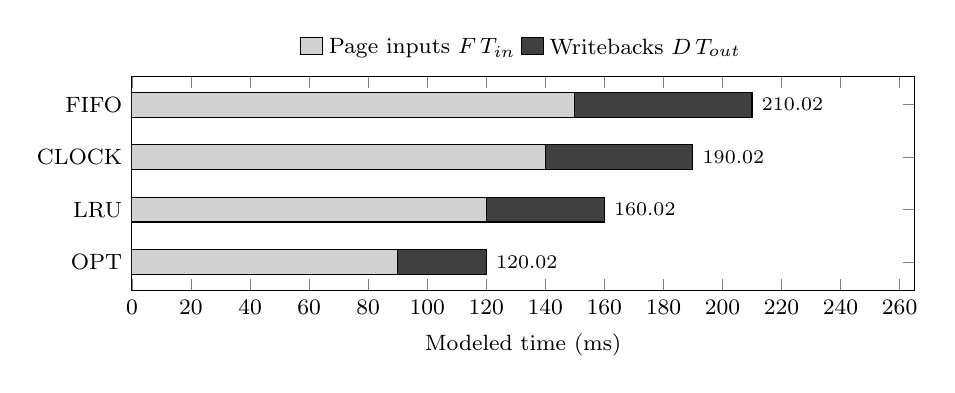
\begin{tikzpicture}
\begin{axis}[xbar stacked, width=0.95\columnwidth, height=4.3cm, bar width=9pt,
  xmin=0, xmax=265, xlabel={Modeled time (ms)}, symbolic y coords={OPT,LRU,CLOCK,FIFO}, ytick=data,
  legend style={at={(0.5,1.03)}, anchor=south, legend columns=2, font=\footnotesize, draw=none},
  tick label style={font=\footnotesize}, label style={font=\footnotesize},
  nodes near coords align={horizontal}, enlarge y limits=0.18]
\addplot[fill=gray!35, draw=black] coordinates {(90,OPT) (120,LRU) (140,CLOCK) (150,FIFO)};
\addplot[fill=black!75, draw=black] coordinates {(30,OPT) (40,LRU) (50,CLOCK) (60,FIFO)};
\legend{Page inputs $F\,T_{in}$, Writebacks $D\,T_{out}$}
\node[font=\scriptsize, anchor=west] at (axis cs:120,OPT) {120.02};
\node[font=\scriptsize, anchor=west] at (axis cs:160,LRU) {160.02};
\node[font=\scriptsize, anchor=west] at (axis cs:190,CLOCK) {190.02};
\node[font=\scriptsize, anchor=west] at (axis cs:210,FIFO) {210.02};
\end{axis}
\end{tikzpicture}
\caption{Composition of the modeled time on Workload A with three frames (simulator output). The reference term $N m = 0.02$\,ms is too small to show.}
\label{fig:cost}
\end{figure}

On Workload~A the order of the policies by modeled time is the same as by fault count: OPT (120{,}020\,$\mu$s), LRU, CLOCK and FIFO (210{,}020\,$\mu$s). Writebacks account for 25 to 29\,\% of the transfer time of each policy, so ignoring them would understate every cost substantially. The fault counts 15, 12 and~9 for FIFO, LRU and OPT equal those of the lecture's page sequence, as expected, because operations never affect victim selection; only $D$ and the cost are new. Evictions equal faults minus the initial fills (three on A).

\section{Student-Designed Tests}\label{sec:tests}
\subsection{Test 1: Dirty State (FIFO, 2 Frames)}
The sequence \code{1:R 1:W 1:R 2:R 3:R 1:R 1:W} was designed to contain a write hit (step~2), a later read of the same page (step~3), a dirty eviction (step~5) and a reload (step~6). Its expected trace was calculated by hand before the program was run and is reproduced exactly (Table~\ref{tab:t1}). The run gives 3 hits, 4 faults (two of them initial fills), 2 evictions, 1 writeback and one resident dirty page at the end; $T_{\mathrm{total}} = 7 + 4 \times 10{,}000 + 10{,}000 = 50{,}007\,\mu$s.

\begin{table}[!tb]
\renewcommand{\arraystretch}{1.05}
\setlength{\tabcolsep}{3.2pt}
\caption{Test 1, dirty state (FIFO, 2 frames): hand-calculated and simulator trace}
\label{tab:t1}
\centering\footnotesize
\begin{tabular}{r c c r c c c c}
\toprule
Step & Ref & H/F & Vic. & WB & F0 & F1 & Hand calc. \\
\midrule
1 & 1:R & F & -- & -- & 1 & -- & \checkmark \\
2 & 1:W & H & -- & -- & 1$^{\ast}$ & -- & \checkmark \\
3 & 1:R & H & -- & -- & 1$^{\ast}$ & -- & \checkmark \\
4 & 2:R & F & -- & -- & 1$^{\ast}$ & 2 & \checkmark \\
5 & 3:R & F & 1 & yes & 3 & 2 & \checkmark \\
6 & 1:R & F & 2 & -- & 3 & 1 & \checkmark \\
7 & 1:W & H & -- & -- & 3 & 1$^{\ast}$ & \checkmark \\
\bottomrule
\end{tabular}
\end{table}

The dirty bit is retained from the first write until the page leaves its frame: the read hit at step~3 does not clear it. It resets only when the page is loaded again (step~6), because the new copy is identical to the backing copy. The writeback is paid when the dirty page is evicted (step~5), not when it is written. The final write (step~7) makes page~1 dirty again; it is still resident at the end and is reported, not flushed.

\subsection{Test 2: Equal Faults, Different Cost (2 Frames)}
The sequence \code{1:R 1:W 2:R 1:R 3:R} was run under all four policies with two frames. Steps 1--4 are identical for all policies and leave page~1 (dirty) and page~2 (clean) resident; step~5 requires a victim (Table~\ref{tab:t2}).

\begin{table}[!tb]
\renewcommand{\arraystretch}{1.1}
\setlength{\tabcolsep}{3pt}
\caption{Test 2: Victim at Step 5 and Cost (Hand-Calculated and Simulator Results Agree)}
\label{tab:t2}
\centering\footnotesize
\begin{tabular}{l p{3.3cm} c c r}
\toprule
Policy & Victim at step 5 & $F$ & $D$ & Total ($\mu$s) \\
\midrule
LRU   & page 2, least recently used (step 3); clean & 3 & 0 & 30{,}005 \\
OPT   & page 1; neither page is used again, tie $\to$ lowest frame index; dirty & 3 & 1 & 40{,}005 \\
FIFO  & page 1, inserted first; dirty & 3 & 1 & 40{,}005 \\
CLOCK & page 1, both bits cleared, hand back at F0; dirty & 3 & 1 & 40{,}005 \\
\bottomrule
\end{tabular}
\end{table}

LRU and OPT incur the same number of faults on the same sequence and capacity, but OPT's modeled time is 10{,}000\,$\mu$s, or 33\,\%, higher because its victim is dirty. A comparison by fault count alone misses this difference, since a dirty eviction adds a writeback that costs as much as a page input; by (\ref{eq:cost}) the cost depends on $F + D$, not on $F$. The comparison is fair only up to the end of the run: LRU leaves page~1 dirty and resident, and that deferred writeback is reported but, by the rules of the model, not charged.

\section{Verification}\label{sec:verif}
Correctness is checked in five ways, summarised in Table~\ref{tab:verif}.

First, after every step the simulator checks that no page is resident twice, that residency never exceeds the capacity, that empty frames are never dirty, that all bits are 0 or~1 and that the CLOCK hand is in range. At the end it checks that hits $+$ faults $= N$, that writebacks $\le$ evictions $\le$ faults, and that evictions $=$ faults $-$ initial fills. A violation stops the program with exit status~3. On Workload~A with FIFO, for example, $5 + 15 = 20$ and $6 \le 12 \le 15$.

Second, the hand-calculated traces of Section~\ref{sec:traces} and both tests of Section~\ref{sec:tests} are stored as expected CSV files and compared row by row with the simulator; on a mismatch the first differing step is printed in both versions. Third, an independent reference model was written in Python from the rules alone, using different data structures (an explicit FIFO queue and an LRU recency list); on 2{,}000 random workloads generated with a fixed seed (1--8 frames, up to 60 references, all four policies) every trace row and counter agrees. Fourth, thirteen invalid inputs must be rejected with an explanation, and a run with 256 references and 64 frames must be accepted. Fifth, to confirm that these tests can detect errors, five typical mistakes were injected into copies of the simulator (Table~\ref{tab:mut}); each was detected, with the first differing decision reported.

\begin{table}[!tb]
\renewcommand{\arraystretch}{1.1}
\caption{Results of the Automated Checks}
\label{tab:verif}
\centering\footnotesize
\begin{tabular}{l r r}
\toprule
Check group & Checks & Passed \\
\midrule
Hand-calculated traces (6 required runs, 3 test runs) & 9 & 9 \\
Summaries and costs of tests and runs & 6 & 6 \\
Rejection of invalid input (13) and limit case (1) & 14 & 14 \\
Differential test, 2{,}000 random workloads & 1 & 1 \\
\midrule
Total & 30 & 30 \\
\bottomrule
\end{tabular}
\end{table}

\begin{table}[!tb]
\renewcommand{\arraystretch}{1.1}
\setlength{\tabcolsep}{3pt}
\caption{Deliberately Injected Mistakes and How They Were Detected}
\label{tab:mut}
\centering\footnotesize
\begin{tabular}{p{2.5cm} c p{3.7cm}}
\toprule
Injected mistake & Failing checks & First differing decision \\
\midrule
Reloaded page keeps old dirty bit & 8 & A--FIFO step 6: page 3 loaded dirty \\
Read clears the dirty bit & 10 & A--FIFO step 5: hit on 0:R cleared page 0's bit \\
LRU not updated on hits & 4 & A--LRU step 6: victim 0 instead of 1 \\
OPT tie to highest index & 3 & Test 2, OPT step 5: victim 2 instead of 1 \\
Writeback for clean victims & 13 & A--FIFO step 4: writeback for clean page 7 \\
\bottomrule
\end{tabular}
\end{table}

\section{Analysis}\label{sec:analysis}
\subsection{Belady's Anomaly in Workload B}\label{sec:belady}
FIFO incurs 9 faults on Workload~B with three frames but 10 with four, so additional memory makes it slower: $T_{\mathrm{total}}$ rises from 90{,}012 to 100{,}012\,$\mu$s. The traces diverge at steps 5 and~6. With four frames these references to pages 1 and~2 are hits, but because FIFO does not refresh insertion age on a hit, pages 1 and~2 remain the oldest pages. From step~7 every fault therefore evicts exactly the page that is needed next (victims 1, 2, 3, 4, 5, 1), and steps 7--12 all fault. With three frames, steps 5 and~6 fault and re-insert pages 1 and~2 as the youngest pages, so after step~7 the frames hold $\{5,1,2\}$ and steps 8 and~9 hit.

The underlying reason is that FIFO is not a stack algorithm: the set of pages resident with three frames is not always a subset of the set resident with four (after step~7, $\{5,1,2\}$ versus $\{5,2,3,4\}$) \cite{belady,silberschatz}. LRU and OPT are stack algorithms, so their fault counts cannot increase with the number of frames. Fig.~\ref{fig:belady}, produced with the simulator for one to six frames, shows this: FIFO (and CLOCK, which behaves identically on this read-only workload) rises from 9 to 10 faults between three and four frames, while LRU falls from 10 to~8 and OPT from 7 to~6.

\begin{figure}[!tb]
\centering
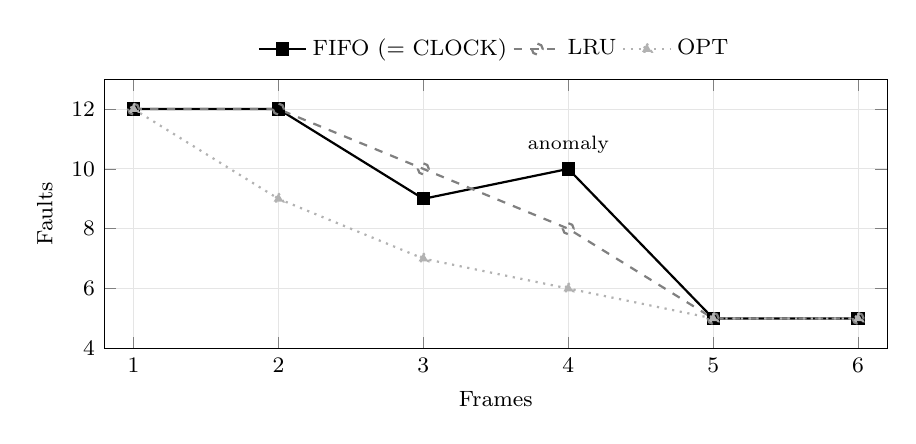
\begin{tikzpicture}
\begin{axis}[width=0.95\columnwidth, height=5cm, xlabel={Frames}, ylabel={Faults},
  xmin=0.8, xmax=6.2, ymin=4, ymax=13, xtick={1,...,6}, ytick={4,6,...,12},
  legend style={at={(0.5,1.03)}, anchor=south, legend columns=3, font=\footnotesize, draw=none},
  tick label style={font=\footnotesize}, label style={font=\footnotesize}, grid=major, grid style={gray!20}]
\addplot[black, thick, mark=square*] coordinates {(1,12) (2,12) (3,9) (4,10) (5,5) (6,5)};
\addplot[gray, thick, dashed, mark=o] coordinates {(1,12) (2,12) (3,10) (4,8) (5,5) (6,5)};
\addplot[gray!60, thick, dotted, mark=triangle*] coordinates {(1,12) (2,9) (3,7) (4,6) (5,5) (6,5)};
\legend{FIFO (= CLOCK), LRU, OPT}
\node[font=\scriptsize, anchor=south] at (axis cs:4,10.2) {anomaly};
\end{axis}
\end{tikzpicture}
\caption{Faults on Workload B as a function of the number of frames (simulator output). Only FIFO shows an increase, from three to four frames.}
\label{fig:belady}
\end{figure}

\subsection{Does OPT Necessarily Have the Lowest Modeled Time?}
No. OPT minimises the number of faults in this model, but it ignores whether its victim is dirty, and its tie-breaking rule prefers the lowest frame index rather than a clean page. On Workload~A OPT is also the cheapest policy (120{,}020\,$\mu$s), because it happens to have the fewest writebacks as well. Test~2 shows the opposite case: OPT and LRU both incur three faults, but OPT evicts the dirty page~1 and LRU the clean page~2, so OPT costs 40{,}005\,$\mu$s and LRU 30{,}005\,$\mu$s. With $T_{in} = T_{out}$, (\ref{eq:cost}) becomes $N m + 10{,}000\,(F + D)$, so a policy with equal or even slightly more faults but fewer dirty evictions can be cheaper than OPT. Minimising faults is therefore not the same as minimising modeled time.

\subsection{Bugs and Rejected Assumptions Exposed by the Tests}
The validation tests exposed two problems in the supplied starter code. Its parser uses \code{strtol}, which skips leading white space and accepts a sign; running the original program as \code{./replacement FIFO 3 +7 " 7" 0} produced an ordinary trace in which both \code{+7} and \code{" 7"} were treated as page~7. Because the assignment requires invalid input to be rejected with an explanation, pages and frame counts are now parsed as decimal digits only, and the test with \code{+7} covers this case. The starter also substituted the lecture sequence when no references were given, whereas the assignment requires a nonempty sequence; an empty sequence is now rejected.

The mutation experiment revealed a less obvious point. Changing OPT's tie-break to the highest frame index passes every check on Workloads A and~B, because no tie between two never-used pages occurs there in a way that changes the result. Only Test~2 and the differential test detect it. The assumption that OPT's tie-breaking rule is irrelevant was therefore rejected: in Test~2 the tie-break alone decides whether a writeback is paid. A further assumption rejected by the model is that a write miss needs no page input; without a whole-page-write optimisation every miss is charged $T_{in}$, as in step~7 of FIFO on Workload~A.

\subsection{The Simplified Model and Linux}
The model assumes one process, a fixed number of frames, serialized transfers with fixed costs, no prefetching, no background writeback and no flush at the end. Linux instead approximates LRU with active and inactive lists, writes dirty pages back in the background before they are reclaimed, reads ahead, and has costs that depend on the storage device and on queueing \cite{silberschatz,ostep}. The simulator results therefore compare policies under identical assumptions; they do not predict the performance of Ubuntu.

\section{Observations on Ubuntu}\label{sec:ubuntu}
\subsection{Environment}
The experiments were run in a browser-based Ubuntu playground (Killercoda), which is a KVM virtual machine (\code{systemd-detect-virt} reports \code{kvm}), accessed from a Mac. The recorded environment is Ubuntu~24.04.5~LTS, kernel 6.8.0-147-generic (x86\_64), page size 4096 bytes, GCC 13.3.0, one virtual CPU, 1.9\,GiB of memory and 1.0\,GiB of swap, none of it in use. Transparent huge pages (THP) were set to \code{madvise} and the use of the huge zero page was enabled; these settings were only read, not changed \cite{thp}. The supplied programs \cite{week6} were used unchanged (their SHA-256 checksums match the course files), the 16\,MiB bound of \code{first-touch.c} was preserved, and both were compiled with the exact commands of the assignment. GCC printed three \code{-Wmisleading-indentation} warnings for lines 19--21 of \code{first-touch.c}, where a loop and the following \code{snapshot()} call share one line; the call runs once after each loop as intended, so the warnings concern layout rather than behaviour. The complete unedited output is included in the source submission (\code{ubuntu/logs/}); Fig.~\ref{fig:log} reproduces the measurements.

\begin{figure}[!tb]
\begin{Verbatim}[fontsize=\scriptsize, frame=single]
$ ./first-touch                    (run 1)
pid=4064 page_size=4096 mapping_bytes=16777216
mapping only       minor_delta=0 major_delta=0
first read         minor_delta=4096 major_delta=0
first write        minor_delta=4096 major_delta=0
repeat write       minor_delta=0 major_delta=0
checksum=0 first_byte=2
   (runs 2, 3: pid=4073, pid=4082;
    all other lines identical to run 1)
$ ./cow-observe                    (runs 1-3)
child_private_value=9 parent_private_value=7
child_private_value=9 parent_private_value=7
child_private_value=9 parent_private_value=7
\end{Verbatim}
\caption{Terminal output of the three runs of each program, abridged from the raw log \code{all\_output.log} in the source submission. All runs exited with status 0.}
\label{fig:log}
\end{figure}

\subsection{First Touch}
\emph{Prediction.} The predictions were recorded before the program was run. The \code{mmap} call only creates a virtual memory area, so the mapping phase should cause about zero faults. A 16\,MiB area contains 4{,}096 pages of 4\,KiB, and the first read of each untouched anonymous page should cause one minor fault, served by mapping the shared read-only zero page; if transparent huge pages were used, one fault could cover 2\,MiB and the count could fall to about~8. Because reading does not allocate private frames, the first write should again cause about 4{,}096 minor faults, and repeated writes about zero. No major faults were expected, because anonymous memory has no file to read and the program is far too small to cause swapping.

\begin{table}[!tb]
\renewcommand{\arraystretch}{1.1}
\setlength{\tabcolsep}{4pt}
\caption{First Touch: Predicted and Observed Fault Increments (Minor / Major)}
\label{tab:ft}
\centering\footnotesize
\begin{tabular}{l c c c c}
\toprule
Phase & Predicted & Run 1 & Run 2 & Run 3 \\
\midrule
Mapping only & $\approx 0$ / 0 & 0 / 0 & 0 / 0 & 0 / 0 \\
First read & $\le 4{,}096$ / 0 & 4{,}096 / 0 & 4{,}096 / 0 & 4{,}096 / 0 \\
First write & $\approx 4{,}096$ / 0 & 4{,}096 / 0 & 4{,}096 / 0 & 4{,}096 / 0 \\
Repeat write & $\approx 0$ / 0 & 0 / 0 & 0 / 0 & 0 / 0 \\
\bottomrule
\end{tabular}
\end{table}

\emph{Observation.} The three fresh processes produced identical increments (Table~\ref{tab:ft}), and each printed \code{checksum=0 first\_byte=2}.

\emph{Interpretation.} The mapping phase caused no faults, confirming that \code{mmap} creates neither frames nor page-table entries until a page is touched. The first read caused exactly $16\,\mathrm{MiB} / 4\,\mathrm{KiB} = 4{,}096$ minor faults, one per page. The checksum of zero shows that every byte read was zero, which is consistent with the reads being served by the zero page without disk access. THP was set to \code{madvise}, and the program does not call \code{madvise}, so 4\,KiB pages were used. The first write caused another 4{,}096 minor faults rather than none: after the read, each page-table entry still referred to the read-only zero page, so every first write faulted, and the kernel allocated a private zero-filled frame---copy-on-write from the zero page. The value \code{first\_byte=2} confirms that both writes reached the private page. Repeated writes caused no faults because the pages were then present, private and writable. No phase caused a major fault, since no file or swap was read.

The counts are not affected by other processes, because \code{getrusage(RUSAGE\_SELF)} counts only the calling process, and the snapshots surround the loops, so faults caused by program start-up or by \code{printf} fall outside the measured phases. The result should nevertheless not be read as a rule of one fault per 4\,KiB. A larger page size (16 or 64\,KiB) would reduce the number of pages, THP set to \code{always} could map the area with 2\,MiB pages and reduce the counts to a few faults, and disabling the zero page or using another kernel could change the read phase. The lecture's macOS counts were not used as a prediction.

\subsection{Copy on Write}
\emph{Prediction.} \code{child\_private\_value=9 parent\_private\_value=7} and exit status~0 in every run.

\emph{Observation.} All three fresh processes printed exactly the predicted line and exited with status~0 (Fig.~\ref{fig:log}).

\emph{Interpretation.} The parent writes 7 into a private anonymous page and then calls \code{fork}. The child receives page tables that refer to the same frame, and the kernel makes both mappings read-only for copy-on-write. When the child writes 9, the write faults and the kernel gives the child a private copy of the page with write permission. The parent's mapping is unaffected, so the parent still reads 7 after the child has exited, and the private writes remain isolated. The printed values cannot show which physical frames were used, whether the two processes ever shared a frame, exactly when the copy was made, or which of the two processes received the new frame; they show only that each process sees its own private value.

\subsection{Prediction Compared with Observation}
Both experiments matched their predictions in every run. For \code{first-touch} the 4\,KiB case predicted for THP in \code{madvise} mode occurred, not the huge-page case; for \code{cow-observe} the values were exactly as predicted. These measurements describe real demand paging and copy-on-write in one environment, whereas the simulator of Sections~\ref{sec:design}--\ref{sec:analysis} is a simplified model; neither is used to predict the numbers of the other.

\section{Conclusion}
The six address cases show that a fault is not necessarily an error: demand paging and copy-on-write repair legal accesses, whereas mapping and protection failures cannot be repaired by free memory. The extended simulator implements FIFO, LRU, OPT and CLOCK with dirty pages and transfer costs according to the rules of the assignment and reproduces all hand-calculated traces; the verification and the injected mistakes indicate that its decisions are correct. The analysis shows that the modeled cost depends on writebacks as well as faults, so that OPT, although optimal in faults, is not always the cheapest policy, and that FIFO exhibits Belady's anomaly on Workload~B. The Ubuntu experiments confirmed lazy allocation, zero-page mapping and copy-on-write as predicted.

\section*{Statement on the Use of AI Assistance}
The conversational AI assistant Claude (Anthropic) was used during this assignment. It explained address translation step by step, which I then applied when solving the six address cases by hand; it reviewed my hand solutions and hand traces and pointed out the gaps described in Sections~\ref{sec:addr} and~\ref{sec:traces}, which I re-traced. It wrote the \code{[A2]} extension of the supplied simulator, the test scripts, the independent reference model and the mutation check; it proposed the two test sequences, which I checked by hand; and it wrote the script for the Ubuntu experiments, drafted the predictions before I ran them, and drafted the text of this report and the README.

The output was checked in several ways. The six required traces were calculated by hand before the program was run and compared with its output row by row; the automated checks, the independent reference model and the injected mistakes are described in Section~\ref{sec:verif}; and every number in this report was taken from the generated traces or from the raw Ubuntu log. I ran the Ubuntu experiments myself. Before that run, the assistant tested the experiment script once in its own sandbox to confirm that it works; that output was discarded and is not used in this report.

One suggestion was corrected and one was rejected. The assistant first suggested running the Ubuntu experiments in GitHub Codespaces, but my account had no free Codespaces usage left, so I used the Killercoda Ubuntu virtual machine instead. The assistant also first produced the report as an online document; I rejected this format in favour of the two-column layout used in Assignment~1.

\begin{thebibliography}{6}
\bibitem{handout} ``CSE513 Assignment 2: Virtual Memory---Predict, Simulate, and Observe,'' course assignment handout, 2026.
\bibitem{silberschatz} A. Silberschatz, P. B. Galvin, and G. Gagne, \emph{Operating System Concepts}, 10th ed. Hoboken, NJ, USA: Wiley, 2018, chs. 9--10.
\bibitem{ostep} R. H. Arpaci-Dusseau and A. C. Arpaci-Dusseau, \emph{Operating Systems: Three Easy Pieces}. Madison, WI, USA: Arpaci-Dusseau Books, 2018, chs. 21--22.
\bibitem{belady} L. A. Belady, R. A. Nelson, and G. S. Shedler, ``An anomaly in space-time characteristics of certain programs running in a paging machine,'' \emph{Commun. ACM}, vol. 12, no. 6, pp. 349--353, 1969.
\bibitem{week6} M. Göktürk, ``CSE513 Week 6 reading,'' course notes, 2026. [Online]. Available: \url{https://www.mehmetgokturk.com/cse513/lecture-06-reading.html}
\bibitem{thp} ``Transparent Hugepage Support,'' \emph{The Linux Kernel Documentation}. [Online]. Available: \url{https://docs.kernel.org/admin-guide/mm/transhuge.html}
\end{thebibliography}

\clearpage
\onecolumn
\section*{Appendix: Scanned Hand Calculations}
The following five pages reproduce the original hand calculations. Sheets 1--3 contain the six address cases (A and B on sheet~1, C and D on sheet~2, E and F on sheet~3); sheet~4 contains the first eight steps of Workload~A under FIFO, LRU, OPT and CLOCK; and sheet~5 contains Workload~B under FIFO with three and four frames.

\begin{center}
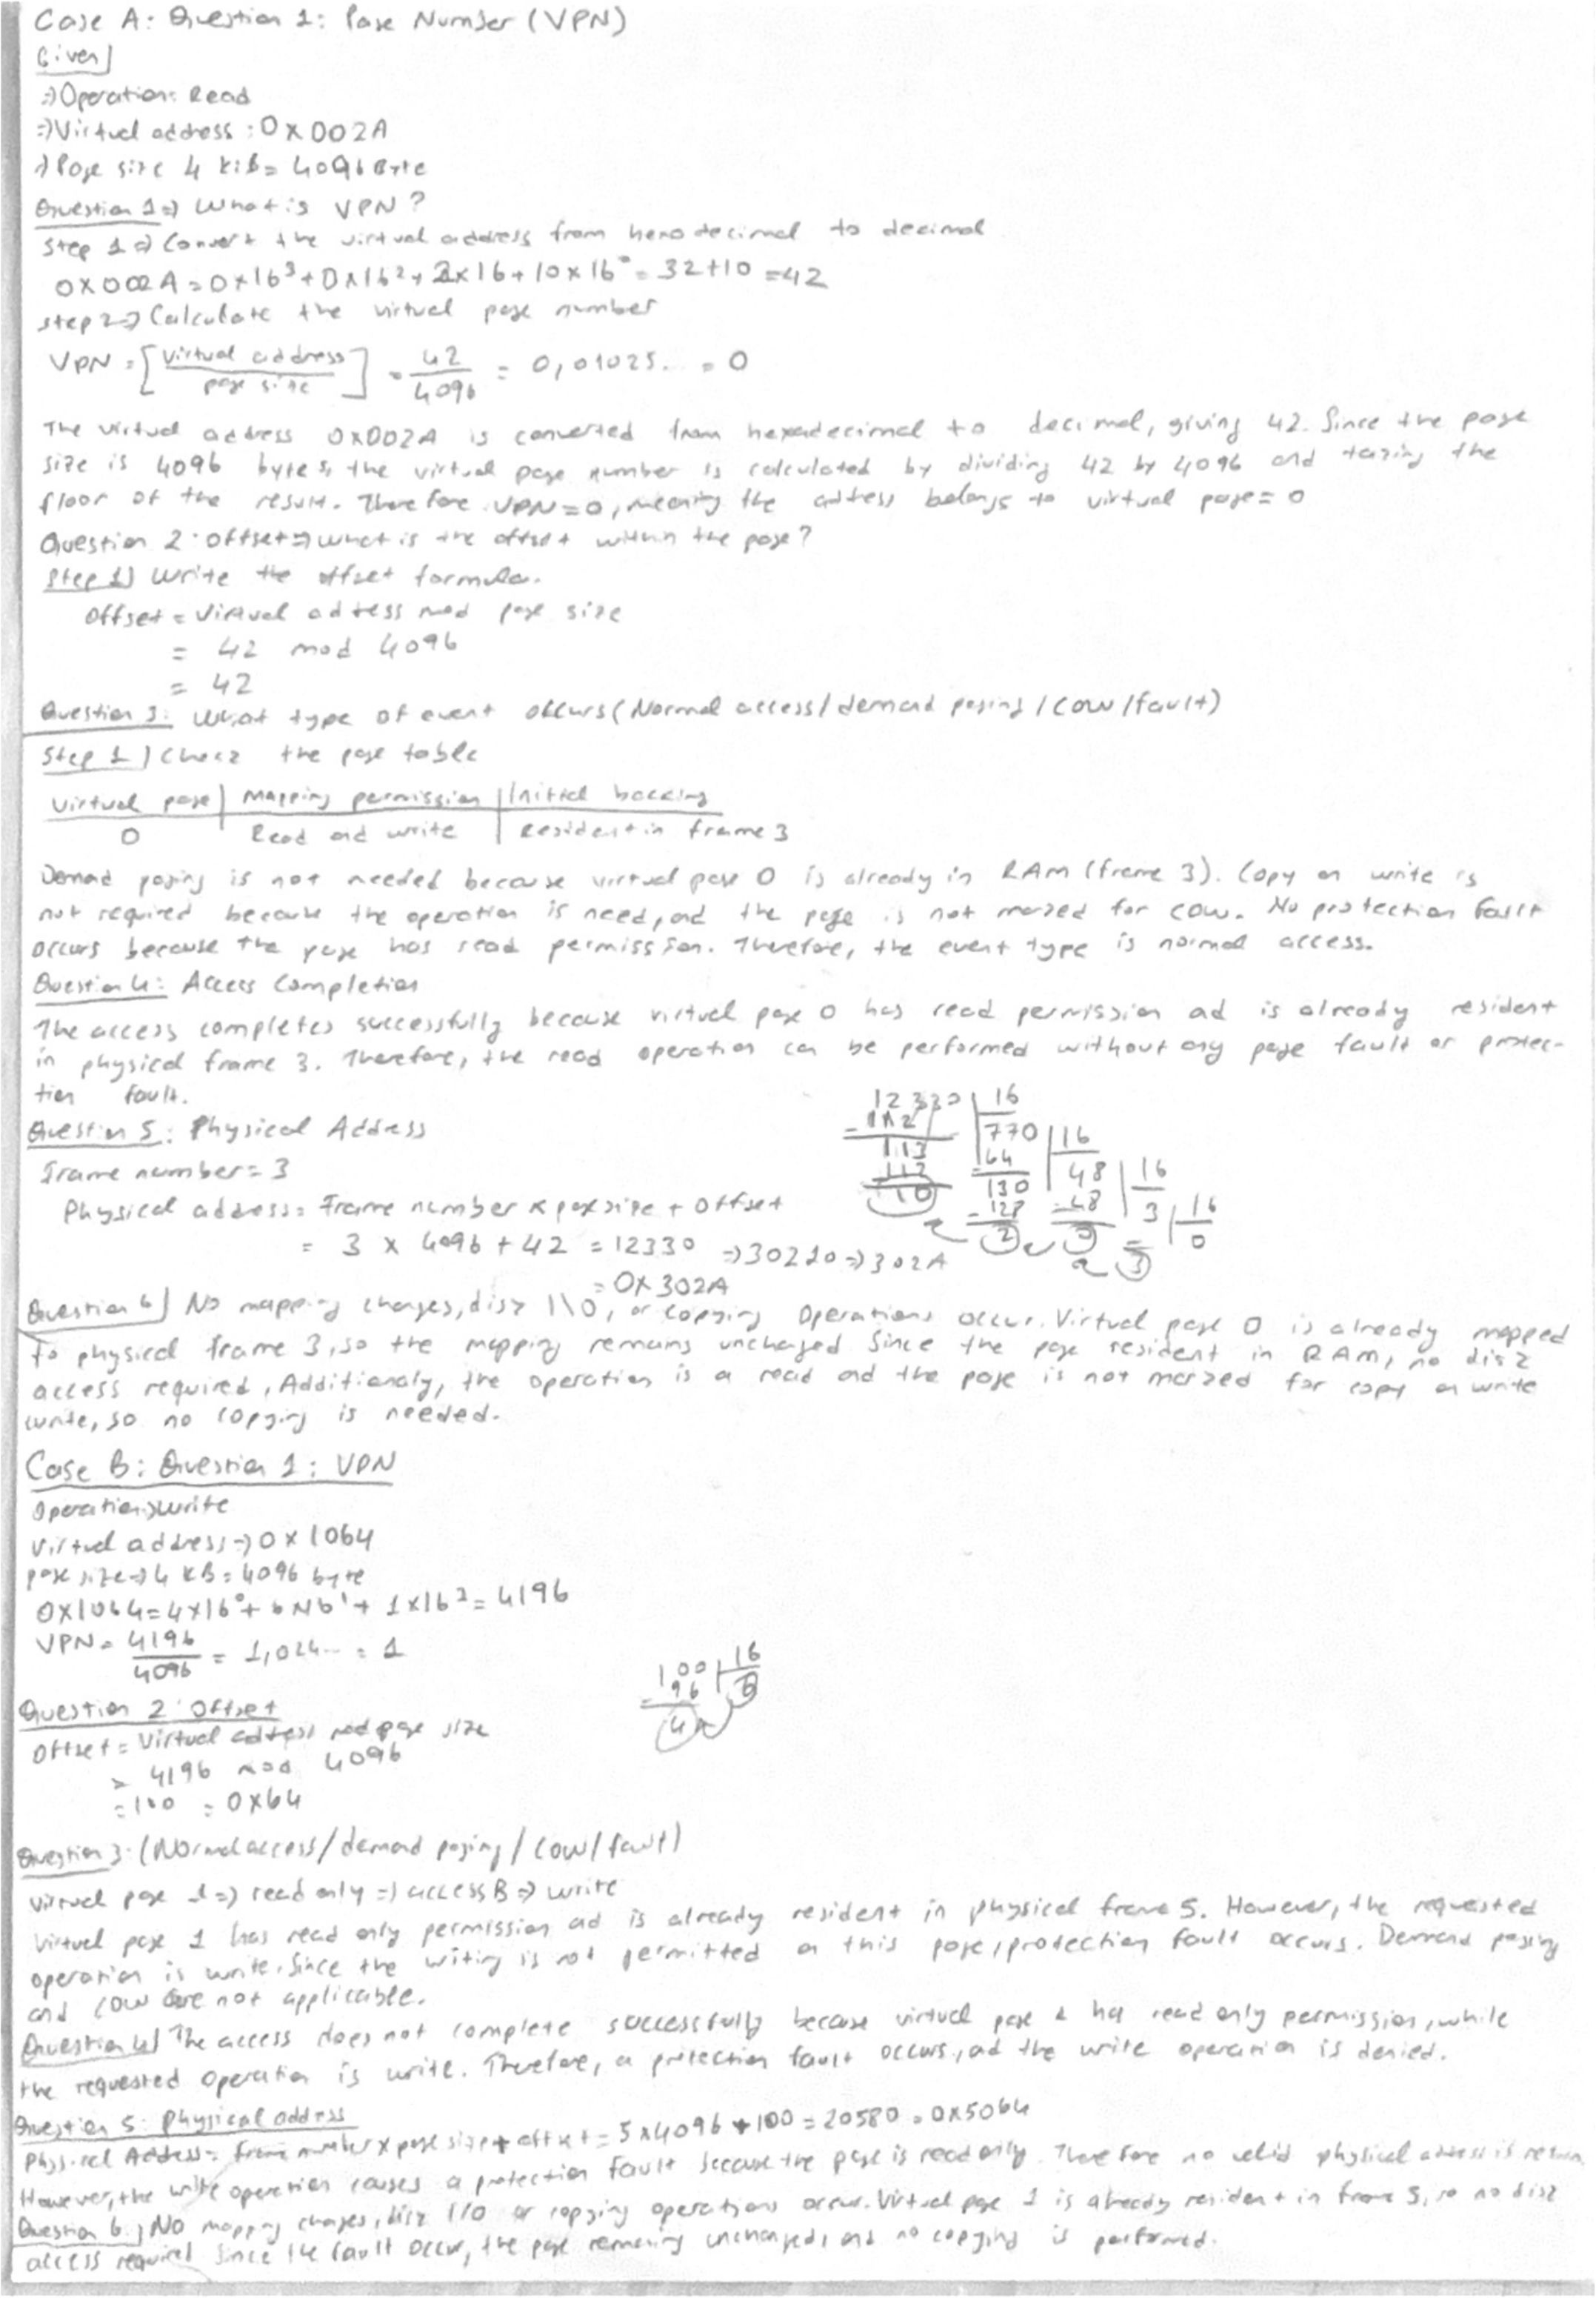
\includegraphics[height=0.86\textheight]{scans/p1-1.jpg}\\[2pt]
{\small Hand-calculation sheet 1: address cases A and B}
\end{center}
\clearpage
\begin{center}
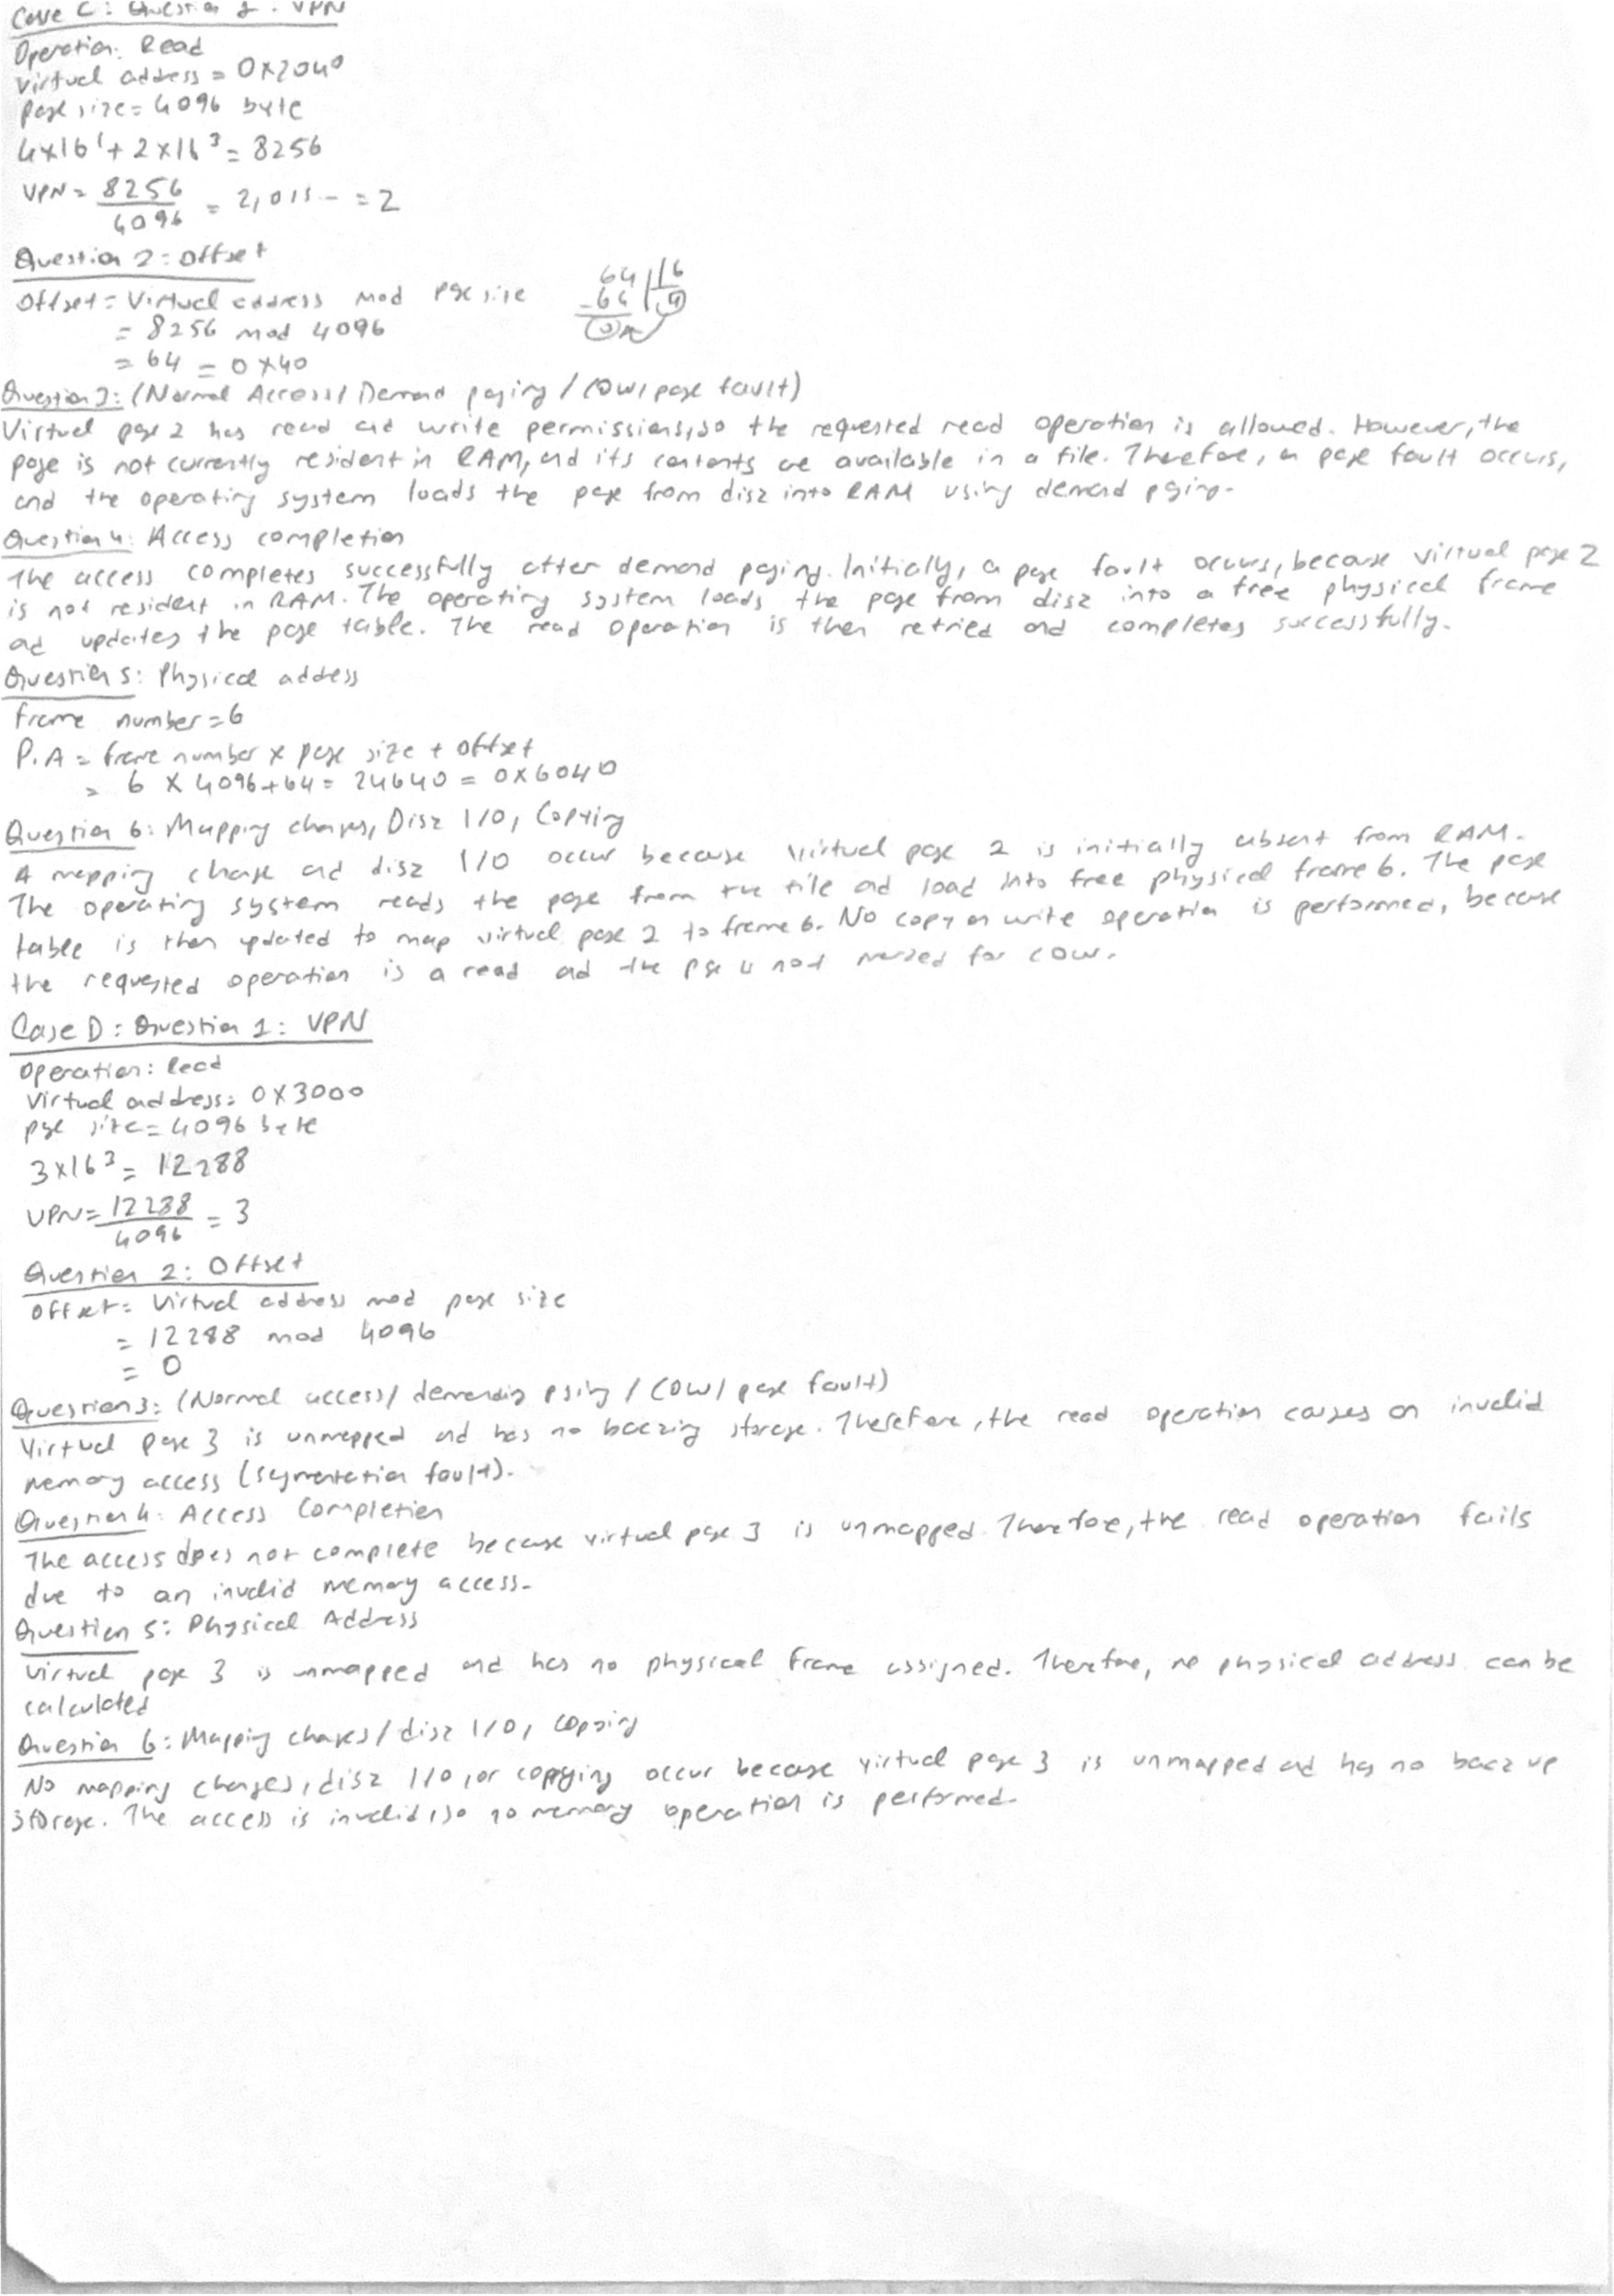
\includegraphics[height=0.88\textheight]{scans/p1-2.jpg}\\[2pt]
{\small Hand-calculation sheet 2: address cases C and D}
\end{center}
\clearpage
\begin{center}
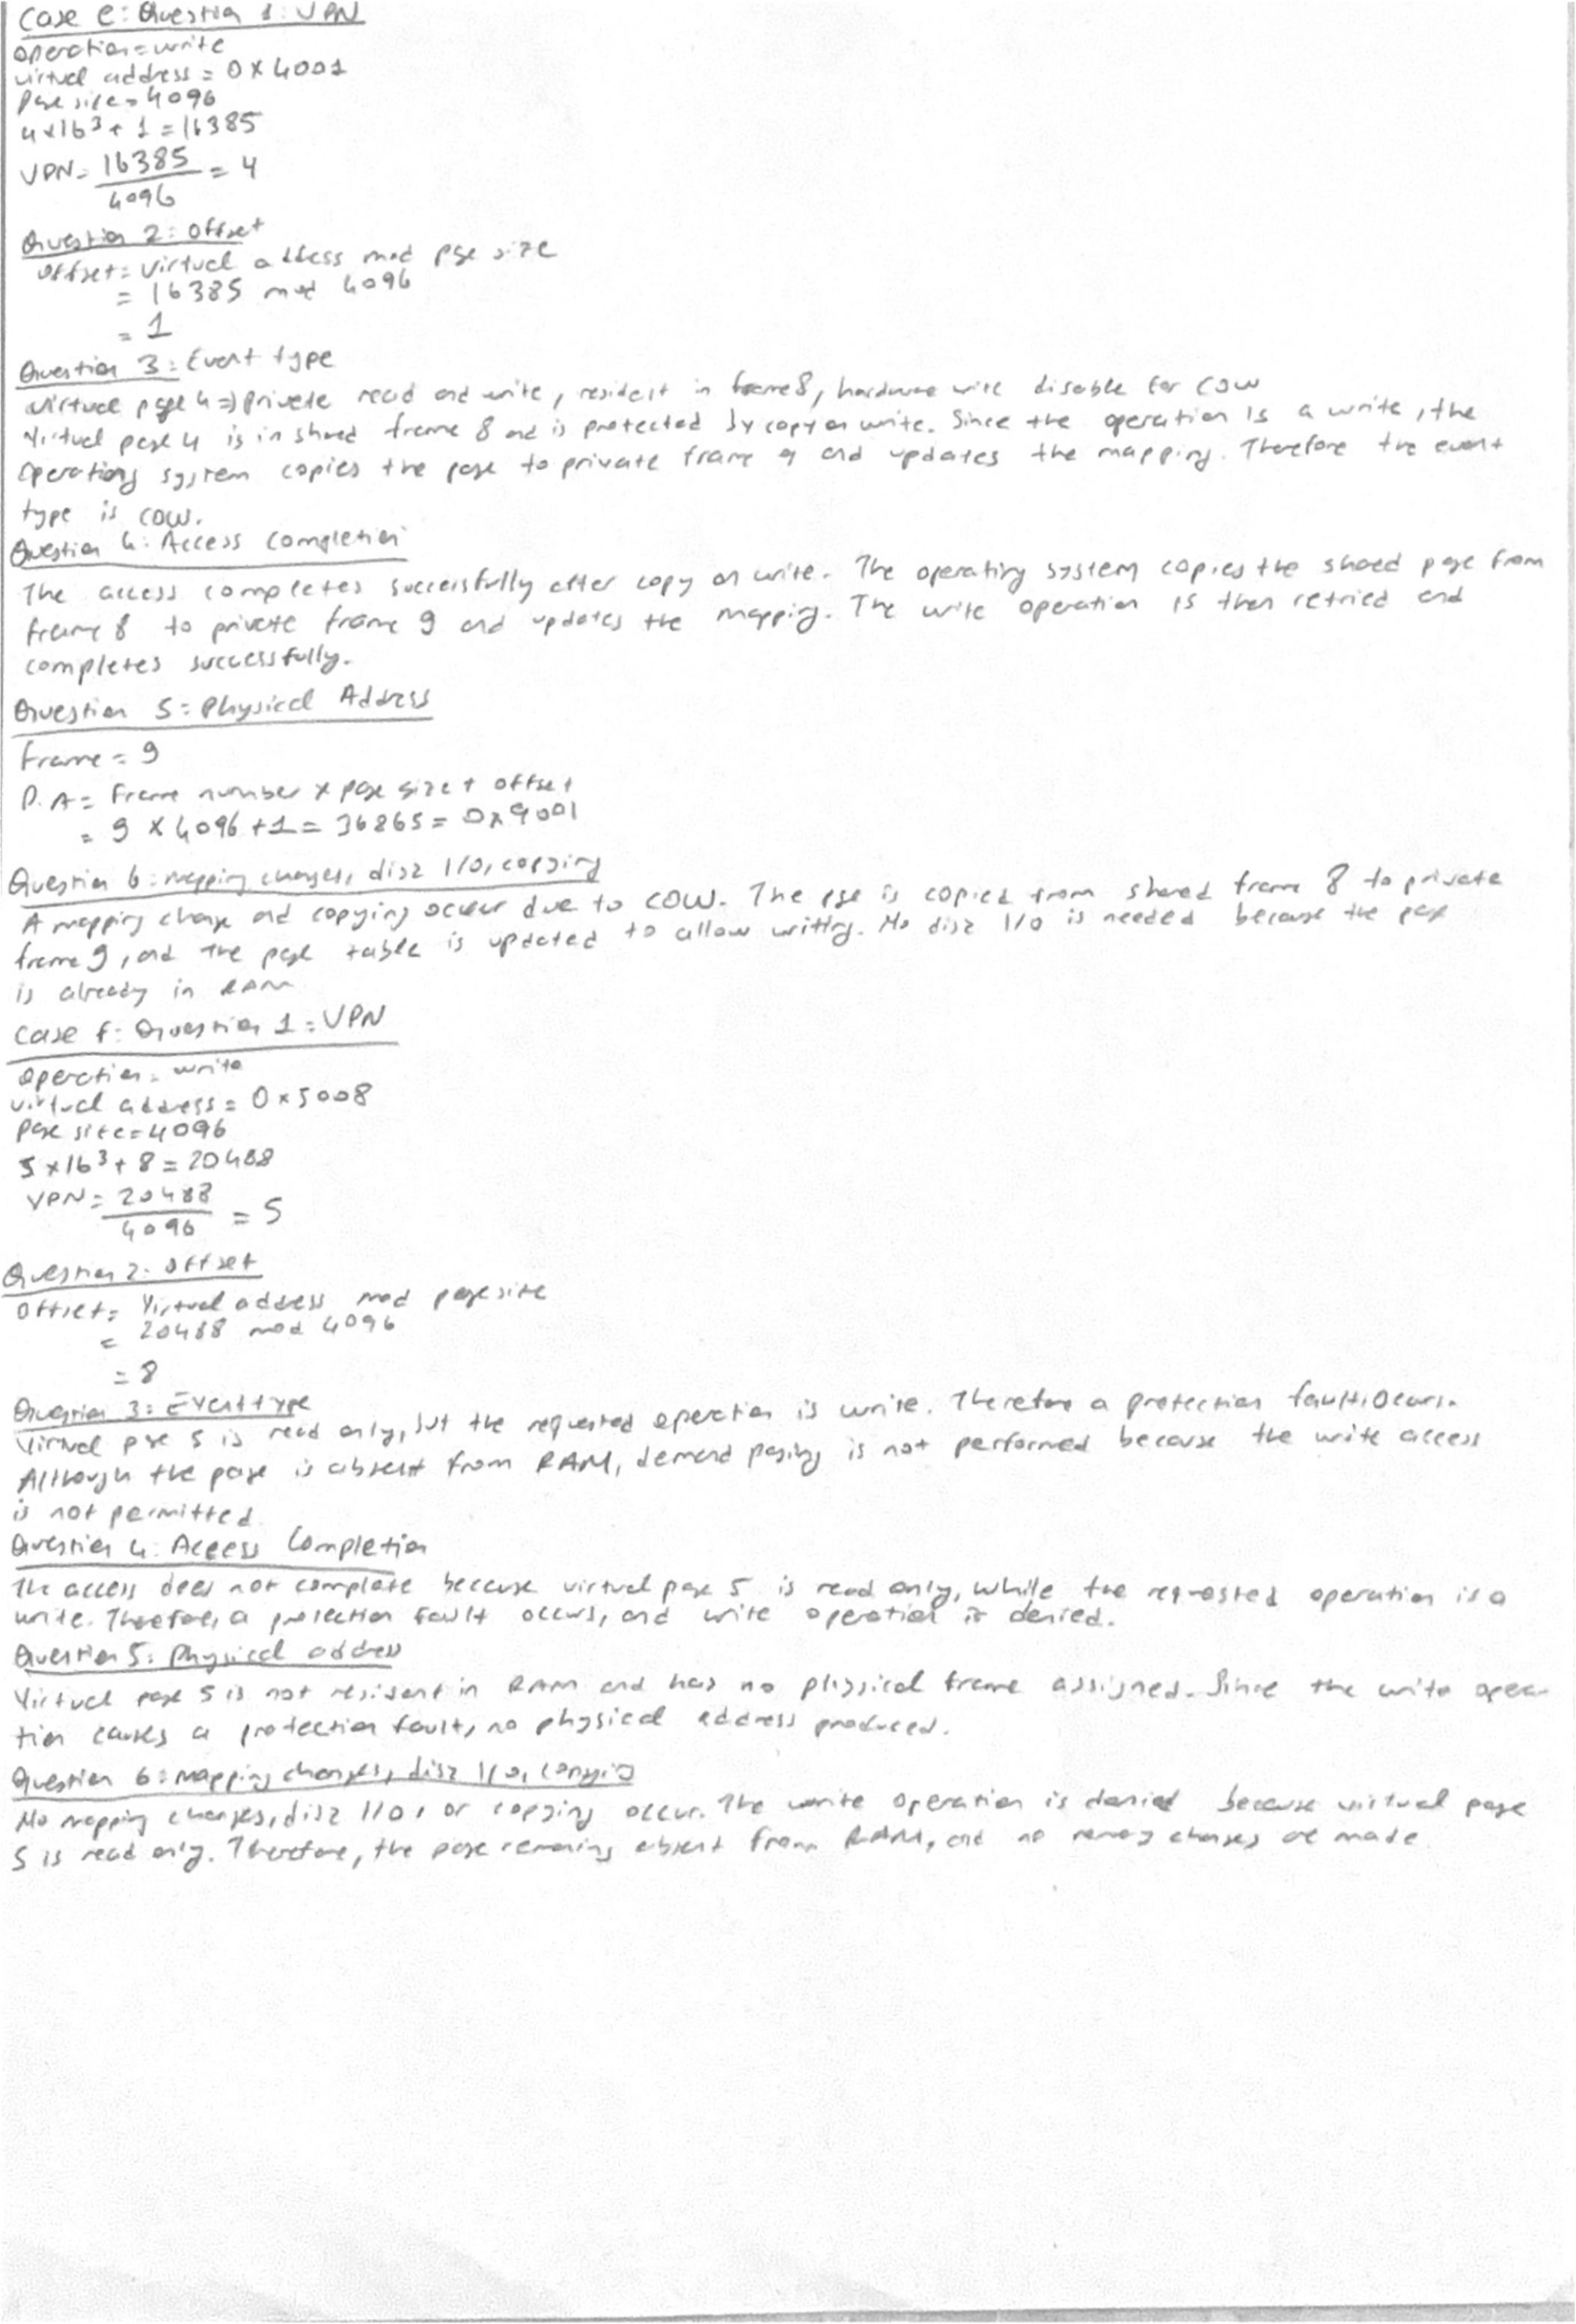
\includegraphics[height=0.88\textheight]{scans/p1-3.jpg}\\[2pt]
{\small Hand-calculation sheet 3: address cases E and F}
\end{center}
\clearpage
\begin{center}
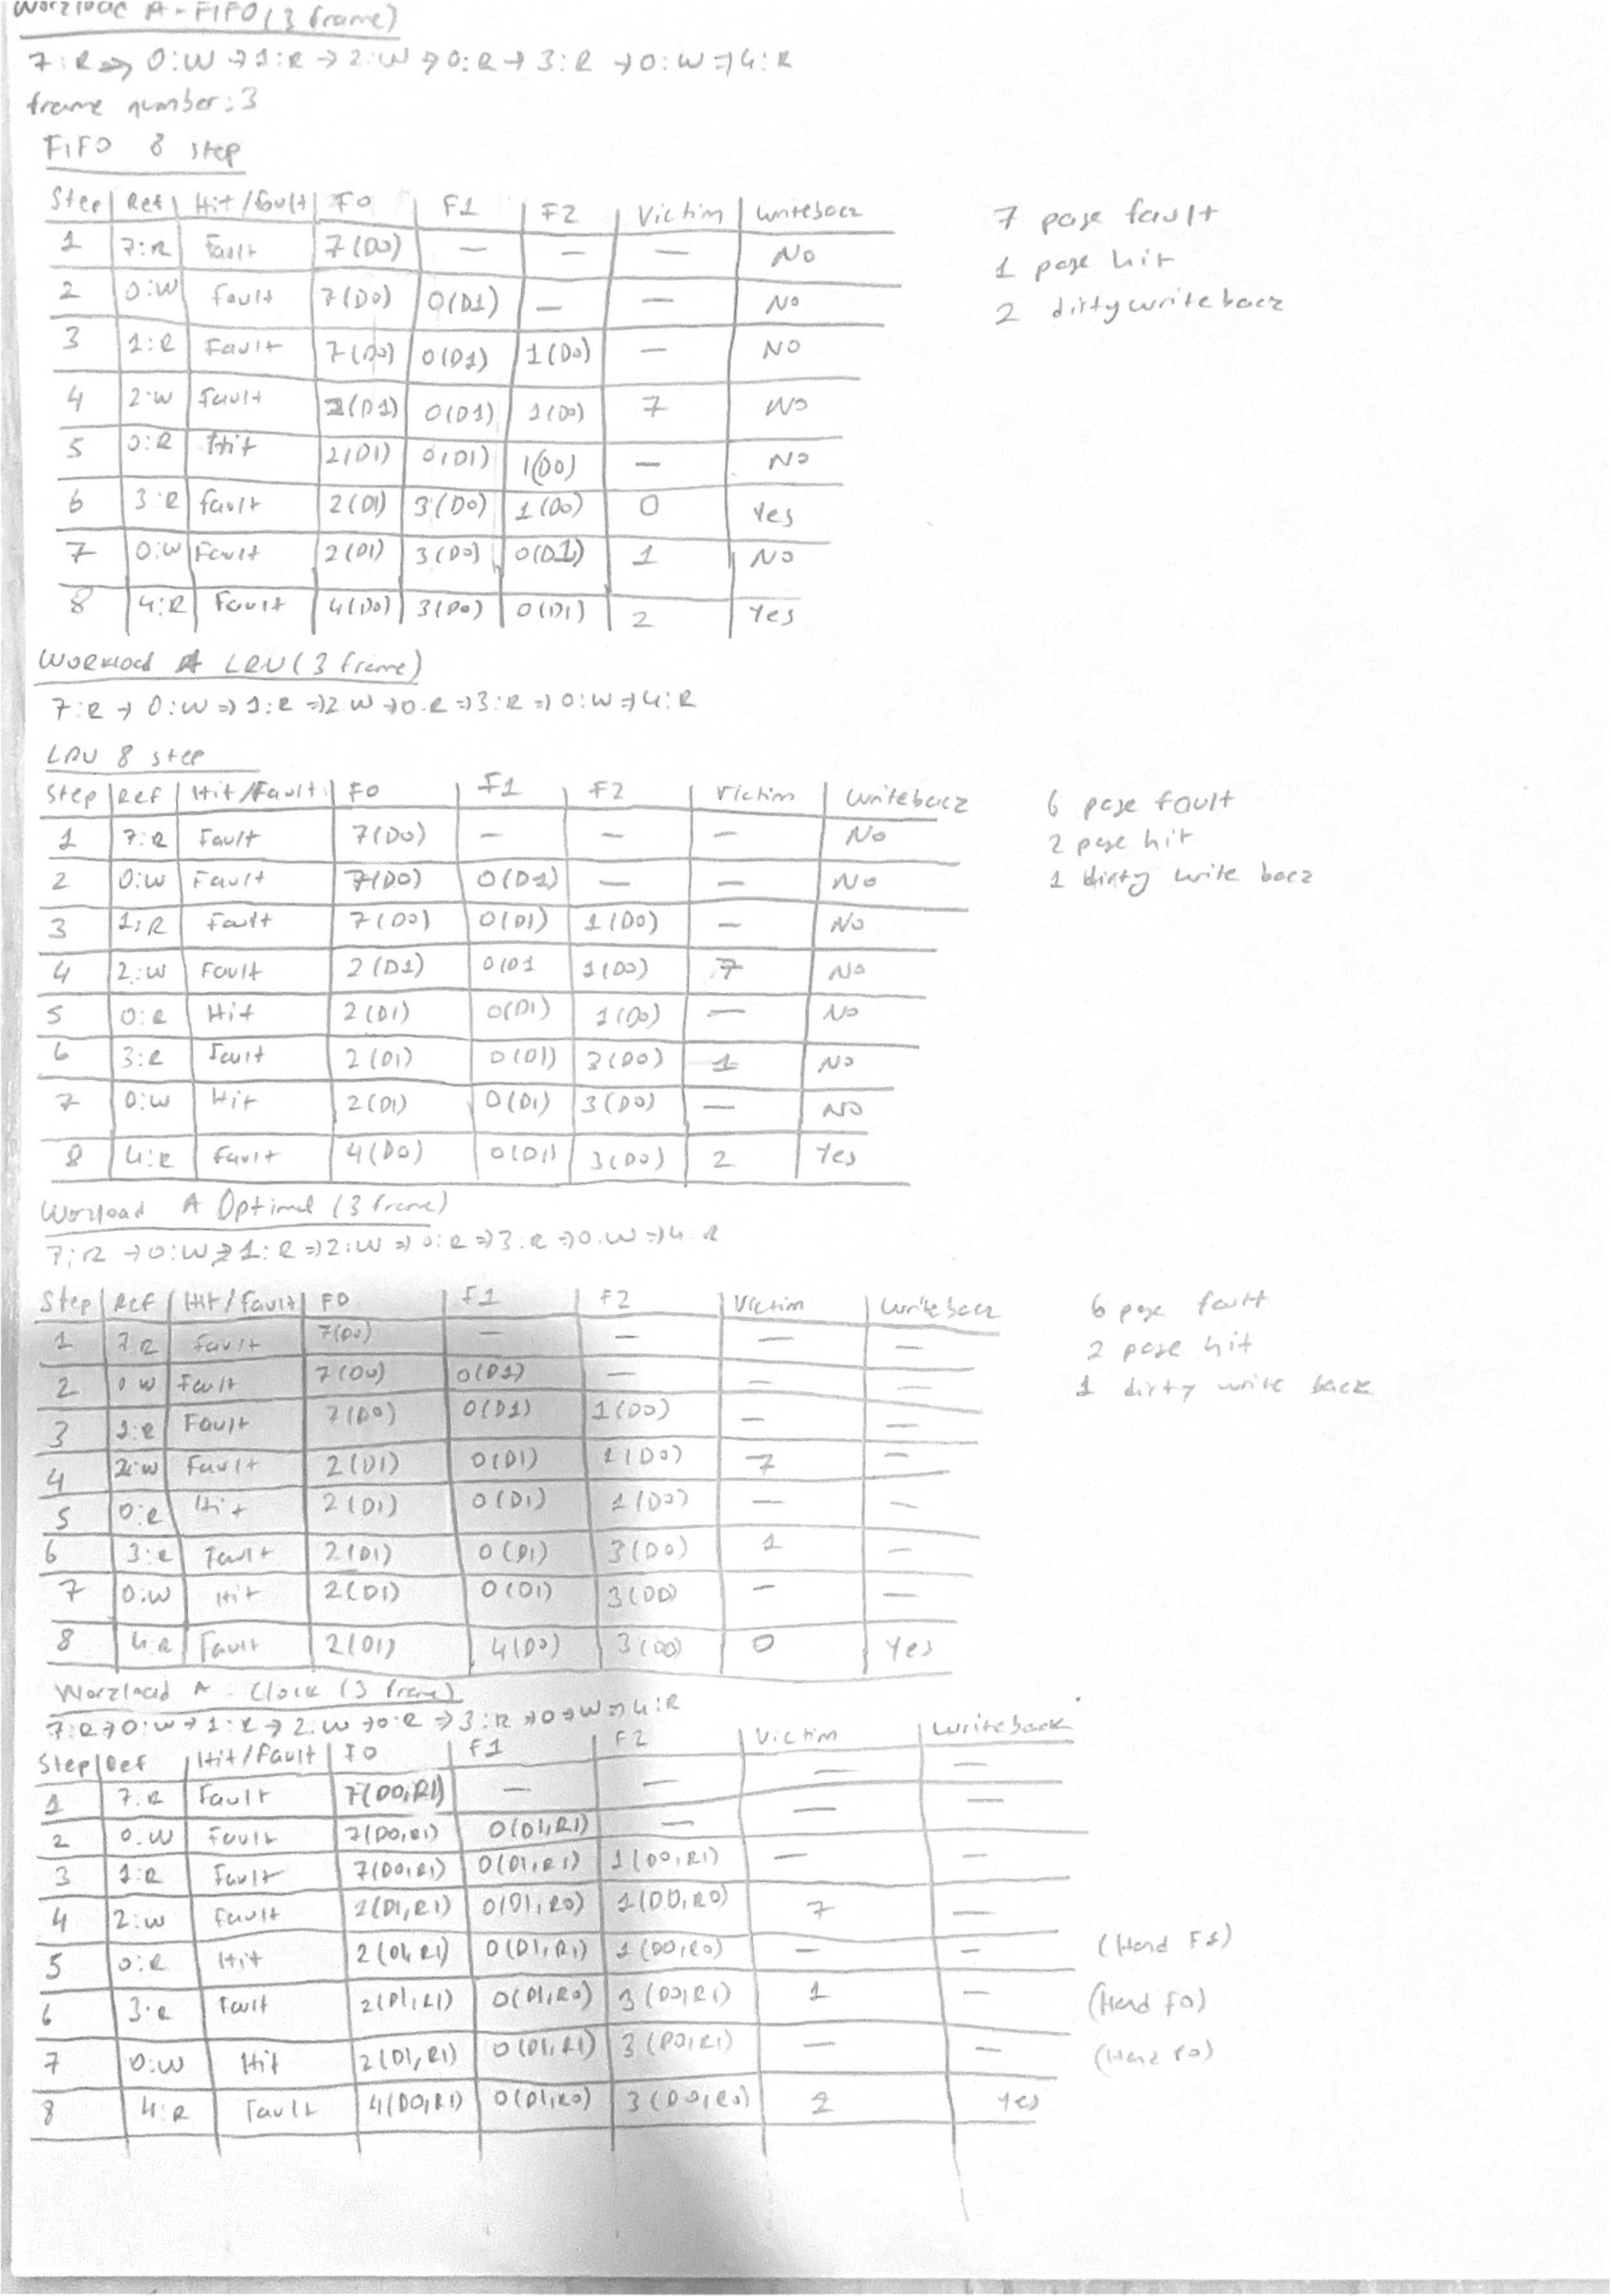
\includegraphics[height=0.88\textheight]{scans/p2-1.jpg}\\[2pt]
{\small Hand-calculation sheet 4: Workload A, first eight steps under FIFO, LRU, OPT and CLOCK (3 frames)}
\end{center}
\clearpage
\begin{center}
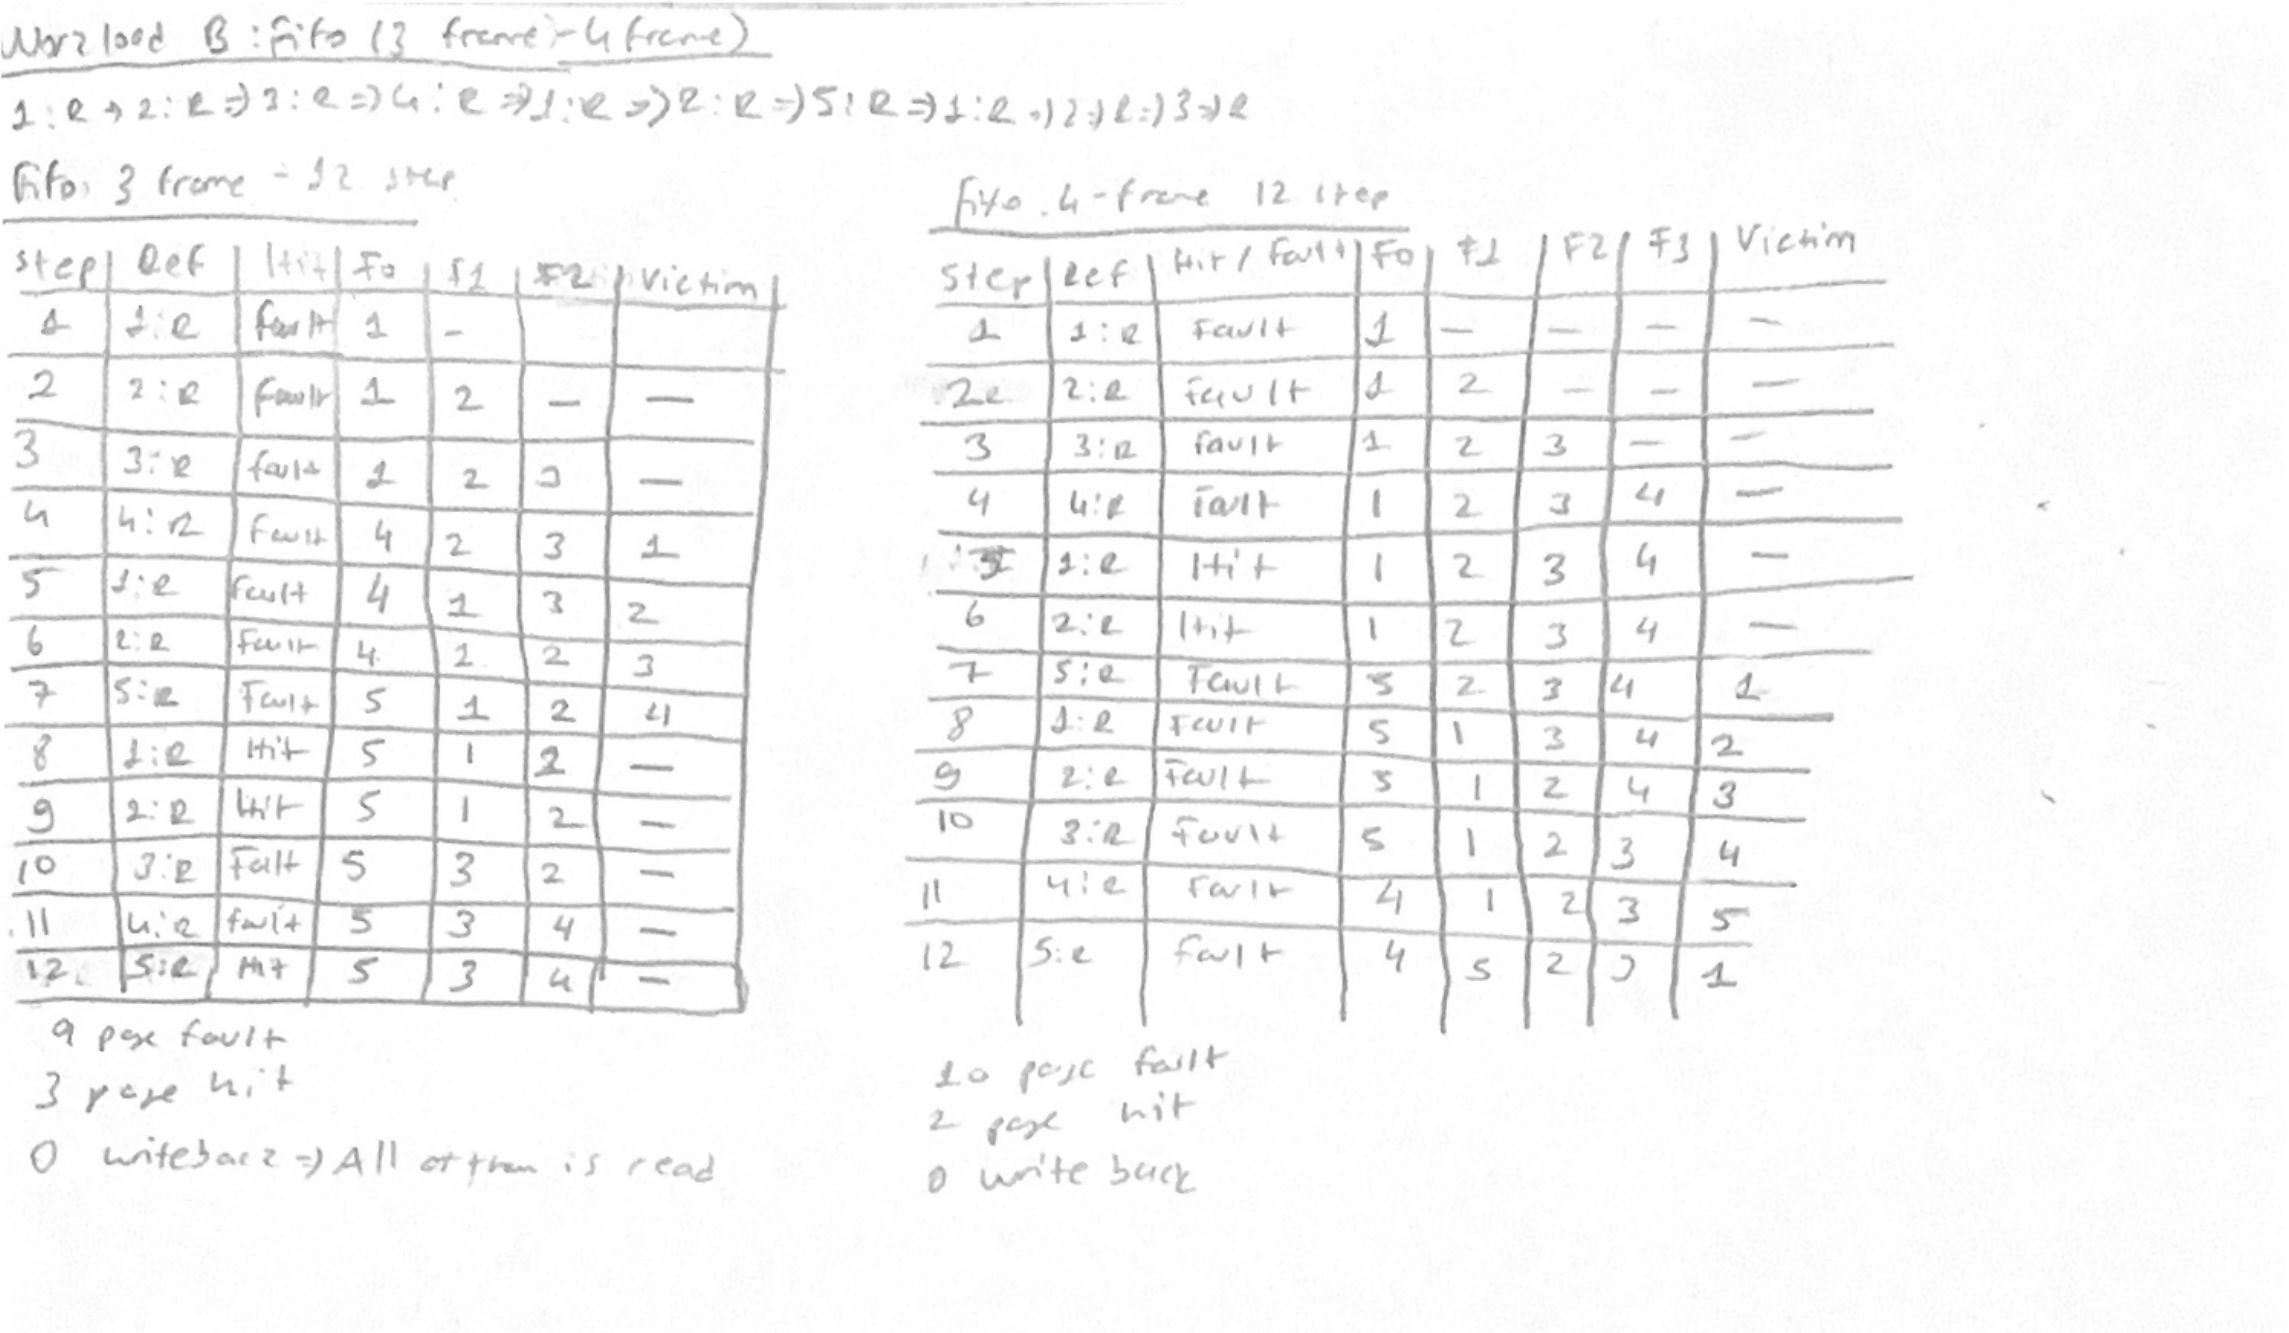
\includegraphics[width=\textwidth]{scans/p2-2.jpg}\\[2pt]
{\small Hand-calculation sheet 5: Workload B under FIFO with 3 and 4 frames}
\end{center}

\end{document}
